\documentclass[11pt,a4paper]{article}
\usepackage[utf8]{inputenc}
\usepackage[T1]{fontenc}
\usepackage{lmodern}
\usepackage{graphicx}
\usepackage{amsmath,amssymb}
\usepackage{booktabs}
\usepackage{array}
\usepackage{geometry}
\usepackage{microtype}
\usepackage[font=small,labelfont=bf]{caption}
\usepackage[colorlinks=true,citecolor=blue,linkcolor=blue,urlcolor=blue]{hyperref}
\geometry{margin=2.4cm}
\graphicspath{{figures/}{.}}

\renewcommand{\topfraction}{0.90}
\renewcommand{\bottomfraction}{0.70}
\renewcommand{\textfraction}{0.08}
\renewcommand{\floatpagefraction}{0.80}

\newcommand{\avg}[1]{\langle #1\rangle}
\newcommand{\Dbar}{\overline{D}}
\newcommand{\Eact}{E_{\mathrm{act}}}
\newcommand{\Plid}{P_{\mathrm{lid}}}
\newcommand{\Sij}{\mathbf{S}}

\title{\bfseries Spatio-temporal wall-actuation modes and cycle-mean\\
viscous dissipation in a lid-driven cavity}

\author{Beniaiche Ahmed$^{1,}$\thanks{Corresponding author: beniaiche\_ahmed25@yahoo.fr}, Larabi Abderrahim$^{1}$, Belkadi Mbarek$^{2}$\\[4pt]
$^{1}$Laboratory of Fluid Mechanics, Ecole Militaire Polytechnique, Algiers, Algeria\\
$^{2}$Laboratory of Turbomachinery, Ecole Militaire Polytechnique, Algiers, Algeria}
\date{}


%-------------------------- marked-up version --------------------------
\usepackage{xcolor}
\newenvironment{chgadd}{\par\begingroup\color{blue}}{\endgroup\par}
\newenvironment{chgdel}{\par\begingroup\color{red}}{\endgroup\par}
%-----------------------------------------------------------------------
\begin{document}
\maketitle

\begin{center}
\fbox{\parbox{0.92\linewidth}{\small
\textbf{Marked-up manuscript.} This file is the revised manuscript with the
changes made relative to the previous version marked. Text in
\textcolor{blue}{blue} is new or rewritten; text in \textcolor{red}{red}
belonged to the previous version and has been removed or replaced. Obsolete
figures and tables of the previous version are not reproduced here; the
corresponding changes are itemised in the response to the editor. Because the
physics-first version is a reorganisation of the paper, most paragraphs carry
a mark.}}
\end{center}
\medskip


\begin{chgdel}
\begin{abstract}
At fixed actuation energy, the lid-driven cavity admits controlled states whose
cycle-mean dissipation differs by up to a factor of three, and the state selected
most often by an optimizer is not the least dissipative. This study asks which
state a physics-informed control of the two-dimensional cavity selects and how
reproducibly. A physics-informed neural network learns the lid velocity in a
truncated spatio-temporal Fourier basis, minimizing viscous dissipation at
prescribed actuation energy for Reynolds numbers between one hundred and one
thousand. At matched energy the first-harmonic control dissipates less than a
uniform lid, whereas the second-harmonic control dissipates more. The sign of
this ordering holds on three grids and against two reference lids; only its
magnitude is reference-dependent. At the same lid speed, by contrast, it lowers
dissipation by seventy-six percent at Reynolds number five hundred and by
eighty-two percent at one thousand, so the two comparisons answer different
questions. Repeated independent trainings yield three converged clusters: a
stationary second-harmonic state, a time-dependent state, and a residual mixture.
A full-spectrum audit adds a first-harmonic class that is empty under variance
regularization. Recovery frequencies depend on Reynolds number, energy,
initialization, loss weights, and control representation. The
variance-regularization weight selects among these states without altering the
Navier--Stokes problem, so the second-harmonic state is regularization-selected
and suboptimal at fixed energy: existence, accessibility, and reproducibility do
not imply energetic optimality.

\medskip\noindent\textbf{Keywords:} physics-informed neural networks; active flow
control; lid-driven cavity; modal branch selection; lattice-Boltzmann method;
reproducibility.
\end{abstract}

%--------------------------------------------------------------
\textbf{Nomenclature}
%--------------------------------------------------------------
\begin{center}
\footnotesize
\renewcommand{\arraystretch}{1.0}
\setlength{\tabcolsep}{2.5pt}
\begin{tabular}{@{}l>{\raggedright\arraybackslash}p{0.78\textwidth}@{}}
\toprule
\multicolumn{2}{@{}l}{\textit{Roman symbols}}\\
\midrule
\(AR\) & cavity aspect ratio, \(L_x/L_y\)\\
\(C_3\) & spectral rank concentration, sum of the three largest control-energy fractions\\
\(D\) & instantaneous viscous dissipation rate, \((2/Re)\int_\Omega \mathbf{S}\!:\!\mathbf{S}\,d\Omega\)\\
\(E_{\mathrm{act}}\) & instantaneous actuation energy of the lid profile, \(\int_0^L U_{\mathrm{lid}}^2\,dx\)\\
\(E_r\) & realized cycle-averaged actuation energy of a transferred control\\
\(E^*\) & prescribed target actuation energy\\
\(f_1,f_2,f_t\) & first-harmonic, second-harmonic, and explicitly time-dependent control-energy fractions\\
\(H_N\) & normalized branch-selection entropy\\
\(K\) & kinetic energy, \(\tfrac12\int_\Omega |\mathbf{u}|^2\,d\Omega\)\\
\(L,L_x,L_y\) & cavity side, streamwise and wall-normal lengths\\
\(N\) & number of lattice nodes per cavity side (LBM resolution)\\
\(P_{\mathrm{lid}}\) & mechanical power injected through the lid, \(\int_0^L U_{\mathrm{lid}}\tau_w\,dx\)\\
\(R_K\) & ratio of fluctuating to mean kinetic energy\\
\(Re\) & Reynolds number, \(U_{\mathrm{ref}}L/\nu\)\\
\(\mathbf{S}\) & strain-rate tensor, \((\nabla\mathbf{u}+\nabla\mathbf{u}^{\mathsf T})/2\)\\
\(t,T\) & time and forcing period\\
\(\mathbf{u}=(u,v)\) & velocity vector and its streamwise/wall-normal components\\
\(u'\) & fluctuating velocity, \(\mathbf{u}-\langle\mathbf{u}\rangle\)\\
\(u'_{\mathrm{rms}}\) & root-mean-square temporal fluctuation at a fixed point\\
\(U_{\mathrm{lid}}\) & lid velocity profile (the actuation)\\
\(U_{\mathrm{ref}}\) & reference velocity, the amplitude of the uniform lid\\
\(U_{\mathrm{SR}}\) & symbolic-regression reconstruction of the mean lid profile\\
\(x,y\) & streamwise and wall-normal coordinates\\
\midrule
\multicolumn{2}{@{}l}{\textit{Greek symbols and branch symbols}}\\
\midrule
\(B_1,B_2,B_3\) & empirical branch classes (second-harmonic dominated, time-dependent dominated, residual)\\
\(B_{\mathrm{first}}\) & first-harmonic branch class of the full-spectrum audit\\
\(\varepsilon\) & integrated viscous dissipation accumulated over an LBM sampling window\\
\(\lambda_{\mathrm{var}}\) & weight of the variance-regularization term of the training loss\\
\(\nu\) & kinematic viscosity\\
\(\tau_w\) & wall shear stress on the moving lid\\
\(\psi\) & stream function\\
\(\omega\) & vorticity\\
\(\omega_{\mathrm{SR}}\) & spatial frequency returned by the symbolic fits\\
\(\Omega\) & cavity domain\\
\midrule
\multicolumn{2}{@{}l}{\textit{Abbreviations}}\\
\midrule
GCI & grid-convergence index\\
LBM & lattice-Boltzmann method\\
LOCO & leave-one-Reynolds-condition-out (cross-validation)\\
MRT & multiple-relaxation-time\\
PINN & physics-informed neural network\\
RMSE & root-mean-square error\\
SR & symbolic regression\\
\bottomrule
\end{tabular}
\end{center}

%--------------------------------------------------------------
\textbf{INTRODUCTION}

%--------------------------------------------------------------

Active flow control seeks to modify fluid motion through externally imposed
actuation in order to achieve a prescribed dynamical or energetic objective,
including drag and lift modification, separation delay, mixing enhancement, and
viscous dissipation reduction~. The difficulty
of this problem arises from the nonlinear and high-dimensional character of the
Navier--Stokes equations: even when the actuator is parameterized by a small number
of degrees of freedom, its interaction with the flow produces multiple competing
responses, strongly non-convex optimization landscapes, and, in many
configurations, multiple stable states. Reviews of flow control and machine-learning-based
fluid mechanics have consequently emphasized the importance of reduced representations,
interpretable flow structures, and systematic treatment of nonlinear effects rather
than relying solely on scalar performance indicators
.
Methodological rigor in reporting convergence outcomes is especially important
when physics-informed or data-driven methods are used, since a single converged
solution may not represent the full landscape of accessible outcomes, and its
physical significance can only be assessed by characterizing how robustly it is
reached and whether it persists under independent numerical scrutiny.

Low-dimensional representations provide a natural route to tractable flow-control
problems. Proper orthogonal decomposition, balanced truncation, dynamic mode
decomposition, resolvent analysis, and related techniques have become standard
tools for identifying dynamically important flow structures and for constructing
reduced-order models amenable to analysis and control
. In control
applications, such representations substantially compress the optimization problem
while retaining structures relevant to the dominant flow response. Reduced-order
optimal-control formulations have been applied to DNS-based flow-control calculations
, and reinforcement-learning methods have
extended this framework to complex geometries including bluff-body drag reduction
. The lid-driven cavity occupies a canonical
position in these investigations: its geometry and boundary conditions are simple,
yet its recirculating flow structure and Reynolds-number dependence provide a
non-trivial test of numerical and physical hypotheses, and high-quality benchmark
solutions are available for independent verification . At
moderate and high Reynolds numbers the uncontrolled cavity develops a rich
sequence of flow structures---corner eddies, secondary recirculations, and an
unsteady shear layer along the moving wall---whose faithful resolution places
stringent demands on the numerical method and on the interpretation of any
optimization outcome .

The energetic physics of this configuration is what makes it a useful test bed.
The lid does work on the fluid at a rate set by the product of the lid velocity
and the wall shear stress, and that work is balanced by viscous dissipation,
which is concentrated in the lid shear layer, in the primary recirculation, and
near the downstream corner where the boundary layer separates. Reshaping the lid
profile therefore changes two things at once: the mechanical power injected into
the cavity, and the spatial distribution of the strain rate at which that power
is dissipated. A control that weakens the corner separation can reduce
dissipation while injecting less power, so that a comparison at fixed lid
velocity and a comparison at fixed actuation energy answer different physical
questions. The first asks whether a given wall motion produces a more efficient
flow; the second asks whether the same energetic budget is spent better. Only
the second is a statement about control efficiency, and it is the one adopted
here. The question addressed below is thus a physical one: among the flow states
that a low-dimensional wall actuation can reach at a fixed energy budget, which
one does the optimization select, and is that state the least dissipative of
them.

Physics-informed neural networks (PINNs) offer an alternative route to
reduced representations~. Rather than
learning a flow response exclusively from precomputed simulation data, PINNs
incorporate the governing differential equations, boundary conditions, and physical
constraints directly into the optimization objective through automatic differentiation
of the network residuals. This formulation is particularly attractive for control
identification because the flow field and the actuation parameters are optimized
simultaneously, allowing the control itself to become an object of analysis rather
than merely an output of a separate surrogate model. Machine learning has been
applied broadly to fluid mechanics for model reduction, turbulence closure, and
optimization~,
and physics-informed variants have demonstrated promising results for laminar,
transitional, and turbulent flows. However, the physics-informed formulation does
not remove the underlying non-convexity of the optimization problem. Different
random initializations, network capacities, loss-weight configurations, regularization
terms, or control parameterizations can lead to qualitatively different converged
states. The repeated appearance of a particular low-dimensional structure cannot,
by itself, establish that the structure is unique, globally optimal, or independent
of the chosen representation.

This issue motivates a distinction that is rarely made explicit in physics-informed
flow-control studies: the distinction between the \emph{existence} of a controlled
branch, its \emph{accessibility} to a particular optimization procedure, and its
\emph{global optimality}. A control branch may be physically realizable and
repeatedly recovered while remaining only one member of a set of competing
converged states. Conversely, a branch that is infrequently recovered may not
be physically less relevant; it may simply be recovered less often
under the adopted optimization formulation. The control parameterization introduces
a further layer of conditioning: a finite basis does not merely reduce the number
of degrees of freedom, but defines the subspace of control space in which the
optimizer searches. An apparently low-dimensional control structure can therefore
reflect both the dynamics of the controlled flow and the geometry of the chosen
optimization space~.
Subcritical non-convex landscapes in fluid mechanics have been characterized for
variational and adjoint-based methods~, and resolvent
analysis has shown how structural assumptions can influence perceived optimal
structures~. A quantitative framework for
distinguishing these contributions is therefore essential before drawing physical
conclusions from a repeatedly observed modal structure.

The present study addresses this branch-selection problem for distributed active
boundary control of the two-dimensional lid-driven cavity. We formulate a
physics-informed optimization in which the Navier--Stokes equations constrain
the flow while a prescribed actuation-energy level and a dissipation-related
objective determine the control. The actuation is represented in a truncated
spatio-temporal Fourier basis, and a parametric neural representation identifies
controls over the investigated Reynolds-number interval. Rather than treating the
dominant modal structure as an assumed optimum, we explicitly test its
recoverability, multiplicity, and parameter dependence. Independent training
realizations estimate empirical branch-selection frequencies
\begin{equation}
\widehat P\!\left(B_i\mid Re,E^*,\lambda_{\mathrm{var}}\right),
\end{equation}
while systematic variations of \(Re\), \(E^*\), network capacity, control-space
truncation, cavity aspect ratio, loss weighting, and control basis determine when
the observed branches persist or change. The resulting branch structure is then
subjected to an independent numerical test: selected controls are transferred
without retraining to an independent multiple-relaxation-time lattice-Boltzmann
(MRT-LBM) solver, providing a completely independent discretization and
implementation. Grid refinement and benchmark comparisons quantify the associated
numerical uncertainty, and symbolic regression provides a compact analytical
approximation enabling assessment of cross-condition generalization. The aim is
a physical account of how a low-dimensional wall motion selects among competing
cavity states, and of what that selection costs in dissipation.

The central questions of this study are therefore: (i) Does a distributed
physics-informed control problem repeatedly select a low-dimensional modal branch
over a range of flow and actuation parameters? (ii) Do independent initializations
reveal competing branches with comparable optimization performance? (iii) How does
the variational structure of the loss redistribute the empirical accessibility of
those branches? (iv) Does the observed modal structure survive changes in the
control representation? (v) Can the resulting branches be independently realized
and distinguished by a conventional numerical flow solver? Answering these questions
provides a more stringent interpretation of low-dimensional structures obtained from
physics-informed optimization and places modal concentration within the broader
framework of nonlinear branch selection in controlled fluid flows. The paper
follows the physics from the flow state to its energy budget.
Section~\ref{sec:problem_and_pinn} formulates the controlled cavity, the actuation
energy that fixes the comparison, and the optimization.
Section~\ref{sec:global_landscape} maps which flow states are reached across the
\((Re,E^*)\) plane. Section~\ref{sec:accessibility} isolates what controls their
accessibility, and Sec.~\ref{sec:robustness} tests whether they survive changes
of capacity, dimension, geometry, and basis. Section~\ref{sec:lbm} transfers the
selected states to an independent solver and measures their dissipation, which
Sec.~\ref{sec:discussion} interprets in energetic terms.
Section~\ref{sec:sr} condenses the dominant mean profile into an algebraic form,
and Sec.~\ref{sec:conclusions} states the conclusions.

%--------------------------------------------------------------
\textbf{PROBLEM FORMULATION AND PHYSICS-INFORMED OPTIMIZATION}

%--------------------------------------------------------------

The objective is to examine how a distributed boundary-control problem can admit
competing low-dimensional actuation branches and how their accessibility changes
with the physical and variational parameters of the identification procedure.
Before introducing the physics-informed optimization, the controlled flow problem
and the admissible actuation space must be specified independently of the neural
network representation. All notation is consistent throughout the paper; additional
implementation details are provided in the Supplementary Material.
\end{chgdel}

\begin{chgadd}
\begin{abstract}
The spatial and temporal organization of wall actuation determines how mechanical
input is distributed across the flow structures of a driven cavity, yet the
resulting viscous-dissipation cost cannot be inferred from the actuation spectrum
or from the time-mean velocity field alone. This study examines the relationship
between wall-actuation structure, hydrodynamic response, and cycle-mean viscous
dissipation in a two-dimensional lid-driven cavity. Stationary harmonic profiles
and three physics-informed actuation branches are transferred to an independent
multiple-relaxation-time lattice-Boltzmann solver and compared at a common
quadratic actuation norm. For stationary controls at $Re=500$, the first spatial
harmonic reduces dissipation by $17.7\%$ relative to a corner-regularized
uniform-lid reference, whereas the second harmonic and the mean profile of the
second-mode-dominated branch increase it by $36.8\%$ and $44.3\%$, respectively.
Grid-refinement and local strain-rate analyses associate this ordering with the
redistribution of dissipation between corner shear layers and the cavity interior.
For time-dependent branches, the cycle-mean dissipation differs markedly from the
dissipation of the time-mean flow. In particular, the temporally dominated branch
has a cycle-mean dissipation approximately $3.1$ times that of the predominantly
stationary branch, despite its much weaker mean-flow contribution. The results
demonstrate that the energetic cost of wall actuation depends on both the spatial
organization and the temporal fluctuations of the resulting flow, and that physical
performance must be assessed using cycle-averaged dissipation rather than modal
accessibility or mean-field diagnostics alone.
\end{abstract}

\noindent\textbf{Keywords:} lid-driven cavity; wall actuation; viscous dissipation;
energy budget; mean-flow diagnostics; mode selection

%----------------------------------------------------------------------
\section{Introduction}
%----------------------------------------------------------------------

Wall actuation is one of the few ways in which the vortical structure of a
confined recirculating flow can be modified without changing its geometry. In a
lid-driven cavity the entire vortex topology is generated by the tangential
motion of a single boundary, so any spatial structure imposed on that boundary
acts directly on the mechanism that sustains the flow. The cavity is therefore a
natural configuration in which to ask a question that is central to flow control
but rarely posed in energetic terms: when two different actuations require the
same control effort, which one produces the less dissipative flow, and why?
The canonical cavity solution and its benchmarks are well established
\cite{ghia1982high,botella1998benchmark,shankardeshpande2000,albensoeder2005accurate,kuhlmann2019},
and the flow has long served as a test bed for control strategies
\cite{gadelhak2000,brunton2015closed}, yet its dissipation budget under
distributed wall actuation has received comparatively little attention.

The energetic mechanism is twofold, and the two parts can act in opposite
directions. Changing the wall velocity changes the mechanical power injected into
the fluid,
$\Plid=\int_0^1 U_{\mathrm{lid}}\tau_w\,dx$, where $\tau_w$ is the wall shear
stress; it also changes the spatial distribution of the strain-rate tensor
$\Sij$, and with it the partition of viscous dissipation between the lid shear
layer, the side-wall layers, the cavity interior and the two upper corners, where
a discontinuous lid produces a stress singularity. A profile can therefore reduce
the peak strain at the corners while increasing the strain everywhere else, and
the net effect is not predictable from the shape of the actuation alone. The
distinction matters because the two natural comparison protocols answer different
questions. Comparing profiles at the same lid-velocity scale
\cite{beniaiche2026} measures what a given actuator amplitude achieves; comparing
them at the same quadratic actuation norm
$\Eact=\int_0^1U_{\mathrm{lid}}^2\,dx$ measures what a given control effort
achieves. The two rankings need not agree, and only the second is a statement
about efficiency. A further distinction, specific to time-dependent actuation, is
that the dissipation of the time-mean field is not the time mean of the
instantaneous dissipation: because $D$ is quadratic in the velocity gradients,
cycle-averaged dissipation always exceeds the dissipation of the mean flow, and
the gap can be orders of magnitude when the fluctuations dominate
\cite{pope2000,landau1987}.

Spatially structured and time-periodic actuations can also support more than one
hydrodynamic response. A periodic boundary-value problem of this type admits
several coexisting branches, and which one is reached depends on the formulation,
the regularization and the initialization of the identification procedure. A
preceding study by Beniaiche \cite{beniaiche2026} investigated the identification
and independent numerical verification of conditional modal collapse in
physics-informed active control of the lid-driven cavity. It established that the
identified actuation is not characterized by a unique, universally selected modal
structure: predominantly stationary second-harmonic controls and strongly
time-dependent alternatives can be recovered depending on initialization,
regularization, and control parameterization. Independent MRT-LBM simulations
further demonstrated that these identified controls can produce physically
distinct cavity responses. The emphasis of that work was on branch identification,
conditional accessibility, and independent numerical reproducibility. The present
study addresses the complementary fluid-mechanical question of how these spatial
and temporal actuation structures affect the viscous-dissipation budget of the
resulting flow. Rather than treating modal recovery as a performance criterion, we
quantify the dissipation of stationary and periodic responses under a common
quadratic actuation norm, distinguish the dissipation of the time-mean field from
the cycle-mean dissipation, and identify the strain-rate distributions responsible
for the observed energetic differences.

The question addressed in this paper is accordingly:
\begin{quote}
How does the spatio-temporal structure of wall actuation determine the cycle-mean
viscous dissipation of the resulting cavity flow at a prescribed
actuation-energy level?
\end{quote}
The sequence of the paper follows that question. Section~\ref{sec:formulation}
fixes the physical and energetic framework, and in particular separates the
quadratic actuation norm from the mechanical power transmitted through the wall.
Section~\ref{sec:modes} defines the stationary modes and the three identified
branches that are compared. Section~\ref{sec:methods} describes how the
actuations are identified and how the flows are computed independently.
Section~\ref{sec:stationary} reports the energetic response of the stationary
modes, Section~\ref{sec:branches} the cycle-mean response of the time-dependent
branches, and Section~\ref{sec:interpretation} interprets both in terms of local
strain and fluctuating gradients. Section~\ref{sec:conclusions} concludes.

%----------------------------------------------------------------------
\section{Physical formulation and energetic framework}
\label{sec:formulation}
%----------------------------------------------------------------------
\end{chgadd}

\subsection{Controlled cavity and governing equations}

\begin{chgdel}
We consider a two-dimensional incompressible lid-driven cavity in which the upper
boundary is subjected to a spatially and temporally distributed tangential actuation.
The lower and lateral walls remain stationary with no-slip conditions. The lid
velocity is not prescribed \emph{a priori} as a uniform profile but is treated as
a control variable drawn from a finite-dimensional admissible space. This is
essential for the subsequent branch analysis: the branches investigated here are
not solutions of different physical problems, but different control-flow realizations
admitted by the same governing equations, boundary geometry, and actuation constraints.

After nondimensionalization by the cavity height \(L_y^{\mathrm{dim}}\), the
wall-normal extent is unity and the streamwise extent equals the aspect ratio
\(AR=L_x^{\mathrm{dim}}/L_y^{\mathrm{dim}}\):
\begin{equation}
0\le x\le L_x,\quad 0\le y\le 1,\quad L_x=AR.
\end{equation}
The reference square cavity corresponds to \(L_x=1\). Velocities are
nondimensionalized by a reference lid velocity \(U_0\), time by
\(L_y^{\mathrm{dim}}/U_0\), and pressure by \(\rho U_0^2\). The Reynolds number is
\begin{equation}
Re=\frac{U_0\,L_y^{\mathrm{dim}}}{\nu},
\end{equation}
where \(\nu\) is the kinematic viscosity. Note that \(U_0\) is a scaling velocity,
not a requirement that the lid remain uniform; the distributed control
\(U_{\mathrm{lid}}\) may change sign locally provided it remains within the
admissible control space and satisfies the prescribed energy constraint.

Two remarks delimit what this boundary condition claims. A tangential velocity
prescribed pointwise along the upper wall is an idealization of actuation hardware
that exists rather than a single rigid lid: an array of independently driven wall
segments reproduces any profile \(U_{\mathrm{lid}}(x)\) up to the segment pitch,
and wall-bounded momentum injection without moving parts is routinely produced by
dielectric-barrier-discharge plasma actuators, whose near-wall body force is
equivalent, in the time-averaged sense used here, to a distributed tangential wall
velocity . What the formulation does \emph{not} assert is that
one rigid translating wall could impose a sign-changing profile; the energy
constraint \(E^\ast\) of Sec.~\ref{sec:control_space} is what keeps the commanded
effort of the distributed actuator in a physically meaningful range. Second, the
optimization is posed in the time-dependent formulation even though the reference
outcome is quasi-stationary. A steady formulation restricts the admissible set to
time-independent lid profiles and would exclude by construction the branch whose
dominant content is temporal (\(B_2\)), so the branch census reported here is only
defined in the unsteady setting; the quasi-stationary \(B_1\) outcome is not an
artifact of that choice, because it is recovered as a stationary state by the
independent LBM verification of Sec.~\ref{sec:lbm}.

The controlled velocity field \(\mathbf{u}=(u,v)\) and kinematic pressure \(p\)
satisfy the dimensionless incompressible Navier--Stokes equations
\begin{equation}
\frac{\partial\mathbf{u}}{\partial t}+(\mathbf{u}\cdot\nabla)\mathbf{u}
=-\nabla p+\frac{1}{Re}\nabla^2\mathbf{u},\quad
\nabla\cdot\mathbf{u}=0.
\end{equation}
The stationary boundaries satisfy the no-slip condition
\begin{equation}
\mathbf{u}=\mathbf{0},\quad x=0,\; x=L_x,\; y=0,
\end{equation}
and the controlled upper boundary satisfies
\begin{equation}
u(x,1,t;Re)=U_{\mathrm{lid}}(x,t;Re),\quad v(x,1,t;Re)=0.
\end{equation}
The problem is nonlinear for two reasons: the Navier--Stokes convective term, and
the boundary condition~?, which is itself selected from a
parameterized control space. The optimization therefore couples the selection of a
boundary actuation to the nonlinear flow response that the same actuation generates.

\textbf{Finite-dimensional spatio-temporal control}

The lid actuation is represented in a truncated spatio-temporal Fourier basis.
The sine basis in \(x\) enforces \(U_{\mathrm{lid}}(0,t;Re)=U_{\mathrm{lid}}(L_x,t;Re)=0\),
preventing discontinuous tangential velocity at the upper corners for every
tested aspect ratio. The cosine basis in \(t\) allows the \(n=0\) terms to
represent purely stationary actuation, the most directly interpretable patterns
physically. The lid velocity is expanded as
\begin{equation}
U_{\mathrm{lid}}(x,t,Re)=\sum_{m=1}^{N_x}\sum_{n=0}^{N_t-1}
a_{mn}(Re)\sin\!\left(\frac{m\pi x}{L_x}\right)\cos(n\pi t).
\end{equation}
The temporal coordinate in Eq.~? is the normalized PINN
time: the residual is imposed on \(t\in[0,1]\), and every cosine factor is evaluated
on that interval. Because the fundamental factor is \(\cos(\pi t)\), the control is
periodic with period \(T=2\) in these units, the \(n\)-th temporal harmonic having
period \(2/n\). The control is therefore exported on the full fundamental period
\(t\in[0,2]\), and the LBM resolves that period with 256 steps, i.e.\ 128 steps per
unit of PINN time. All transient LBM runs of the branch comparison start from rest
(\(\rho=1\), \(\mathbf{u}=\mathbf{0}\)), with the lid switched on at \(t=0\); at
least 200 forced periods are discarded as transient, a drift test on the
cycle-averaged dissipation then fixes the end of the settling phase, and 64
consecutive periods are retained for the statistics. The same initialization, transient
rule and sampling window are used for \(B_1\), \(B_2\) and \(B_3\).
All modal labels use the physical (one-based) convention: the dominant stationary
second spatial harmonic corresponds to \((m,n)=(2,0)\). The baseline control space
uses \((N_x,N_t)=(6,5)\), giving 30 nominal coefficients. Control-space sensitivity
examines
\begin{equation}
(N_x,N_t)\in\{(4,3),(6,1),(6,3),(6,5),(8,5),(8,9)\},
\end{equation}
spanning 6 to 72 nominal modes. The modal energy of coefficient \((m,n)\) is
\begin{equation}
\mathcal{E}_{m0}=\tfrac{1}{2}a_{m0}^2,\quad
\mathcal{E}_{mn}=\tfrac{1}{4}a_{mn}^2\quad(n\ge1),
\end{equation}
where the factors account for temporal basis normalization
(\(\langle\cos^2(0)\rangle=1\), \(\langle\cos^2(n\pi t)\rangle=\tfrac{1}{2}\) for \(n\ge1\)).
The normalized modal fraction is
\begin{equation}
f_{mn}=\frac{\mathcal{E}_{mn}}{\displaystyle\sum_{i=1}^{N_x}\sum_{j=0}^{N_t-1}\mathcal{E}_{ij}},
\qquad\sum_{m=1}^{N_x}\sum_{n=0}^{N_t-1}f_{mn}=1.
\end{equation}
The stationary second-harmonic fraction is \(f_2\equiv f_{20}\), and the total
time-dependent fraction is \(f_t=\sum_{m=1}^{N_x}\sum_{n=1}^{N_t-1}f_{mn}\).
The realized actuation energy is
\begin{equation}
E_r=\langle U_{\mathrm{lid}}^2\rangle_{s,t}
=\frac{1}{T}\int_0^T\!\!\int_0^1 U_{\mathrm{lid}}^2(s,t;Re)\,ds\,dt,
\quad s=\frac{x}{L_x},
\end{equation}
and the optimization is conditioned on \(E_r\approx E^*\). Modal-energy quadrature
conventions are detailed in Supplementary Sec.~S2.

\textbf{Parametric PINN formulation}

The flow field and Reynolds-dependent control coefficients are represented
simultaneously by a parametric neural network with inputs \((x,y,t,\widetilde{Re})\),
where
\begin{equation}
\widetilde{Re}=\frac{Re-550}{450}\in[-1,1],
\end{equation}
maps the training interval \([100,1000]\) to \([-1,1]\). A single trained network
represents the flow-control pair over the entire Reynolds-number range, enabling
efficient evaluation of the branch map without repeated retraining at each condition.
The flow variables \((u,v,p)\) and control coefficients \(\{a_{mn}(\widetilde{Re})\}\)
are the network outputs. Two subnetworks are employed: a flow network with 6 hidden
layers of 64 neurons each using \(\tanh\) activation (21\,379 trainable parameters),
and a control network with 4 hidden layers of 32 neurons each (3\,614 parameters).
All computations are performed in double-precision arithmetic, and all physical
residuals are evaluated by automatic differentiation. Full architecture
specifications are provided in Supplementary Sec.~S1.

\textbf{Optimization objective and training procedure}

The multi-objective loss is
\begin{equation}
\mathcal{L}=\lambda_{\mathrm{PDE}}\mathcal{L}_{\mathrm{PDE}}
+\lambda_{\mathrm{BC}}\mathcal{L}_{\mathrm{BC}}
+\lambda_{\mathrm{diss}}\mathcal{L}_{\mathrm{diss}}
+\lambda_{\mathrm{ctrl}}\mathcal{L}_{\mathrm{ctrl}}
+\lambda_{\mathrm{var}}\mathcal{L}_{\mathrm{var}}
+\lambda_{Re}\mathcal{L}_{Re},
\end{equation}
with reference weights
\(\lambda_{\mathrm{PDE}}=1,\; \lambda_{\mathrm{BC}}=15,\;
\lambda_{\mathrm{diss}}=0.05,\; \lambda_{\mathrm{ctrl}}=200,\;
\lambda_{\mathrm{var}}=1,\; \lambda_{Re}=2\).
The individual loss components are:

\textbf{PDE residual loss:}
\(\mathcal{L}_{\mathrm{PDE}}=\langle R_u^2+R_v^2+R_c^2\rangle_{\mathcal{X}_{\mathrm{int}}}\),
where \(R_u,R_v,R_c\) are momentum and continuity residuals evaluated at
\(N_{\mathrm{phys}}=4\,000\) interior collocation points resampled uniformly at each epoch.

\textbf{Boundary condition loss:}
\(\mathcal{L}_{\mathrm{BC}}=\langle u^2+v^2\rangle_{\Gamma_{\mathrm{stat}}}
+\langle[u-U_{\mathrm{lid}}]^2+v^2\rangle_{\Gamma_{\mathrm{top}}}\),
where \(\Gamma_{\mathrm{stat}}=\{x=0\}\cup\{x=L_x\}\cup\{y=0\}\). The weight
\(\lambda_{\mathrm{BC}}=15\) enforces boundary conditions strongly relative to
the interior residual.

\textbf{Viscous dissipation objective:}
\begin{equation}
\mathcal{L}_{\mathrm{diss}}=\int_\Omega\frac{1}{Re}
\!\left[u_x^2+v_y^2+\tfrac{1}{2}(u_y+v_x)^2\right]d\Omega
=\int_\Omega\nu\,S{:}S\,d\Omega.
\end{equation}
This term drives the optimizer toward low-dissipation actuation patterns and
constitutes the physical objective of the control problem. Here
\(S_{ij}=\tfrac12(\partial_i u_j+\partial_j u_i)\) is the strain-rate tensor, so
\(\mathcal{L}_{\mathrm{diss}}\) equals exactly half the standard integrated
dissipation rate \(\varepsilon=2\nu S{:}S\) reported by the independent LBM
diagnostic; the factor of two is absorbed by \(\lambda_{\mathrm{diss}}\) and does
not affect the optimum.

\textbf{Actuation energy penalty:}
\(\mathcal{L}_{\mathrm{ctrl}}=(E_r-E^*)^2\). The large weight
\(\lambda_{\mathrm{ctrl}}=200\) enforces the energy budget tightly, ensuring that
competing converged solutions are compared at the same actuation energy level and
that the modal competition is not trivially explained by different energy budgets.

\textbf{Variance regularization:}
\begin{equation}
\mathcal{L}_{\mathrm{var}}=-\log\!\left[\operatorname{Var}(U_{\mathrm{lid}})+10^{-5}\right].
\end{equation}
This term penalizes spatially uniform or near-uniform lid profiles by rewarding
higher spatial variance. It plays a critical role in breaking degeneracy toward
trivially flat controls and is the primary determinant of branch selection, as
demonstrated in Section~\ref{sec:accessibility}.

\textbf{Reynolds-separation regularization:}
\begin{equation}
\mathcal{L}_{Re}=\max\!\left[0,\;\delta-
\frac{1}{N_{\mathrm{probe}}}\sum_{i=1}^{N_{\mathrm{probe}}}
\!\left(U_{\mathrm{lid}}(x_i,t_0,Re_{\min})
-U_{\mathrm{lid}}(x_i,t_0,Re_{\max})\right)^2\right],
\end{equation}
with \(N_{\mathrm{probe}}=20\), \(t_0=0.5\), \(\delta=0.01\), preventing the
parametric network from collapsing to a Reynolds-independent control.

No initial-condition term appears in Eq.~?, and this omission
is deliberate. Because the flow and the control are expanded in a temporal Fourier
basis and the objective is a cycle-averaged dissipation at a prescribed actuation
energy, the network is formulated as a periodic space--time boundary-value
problem: it seeks a statistically stationary, time-periodic state compatible with
the wall boundary conditions, not the transient evolution from a prescribed
initial field. The word ``initialization'' in this work therefore refers to the
initialization of network parameters, never to a flow initial condition. The PINN
results consequently characterize which periodic state a training protocol
reaches, not how long a physical flow takes to reach it from rest, and they carry
no phase information relative to a physical initial time. The independent LBM
calculations used for verification do start from rest and discard at least 200
periods before sampling (Sec.~\ref{sec:lbm}), so initial-value behavior is checked
there rather than assumed for the PINN.

Training consists of a 300-epoch pre-training phase in which only the flow network
is updated with control coefficients frozen at zero, establishing an initial
physically consistent flow representation. A 3\,000-epoch joint optimization phase
follows using the Adam optimizer with initial learning rate \(\eta_0=8\times10^{-4}\)
and exponential decay by factor \(0.995\) per 100 epochs. Collocation points are
resampled at every epoch. Complete sampling details are provided in
Supplementary Sec.~S1.

\textbf{Branch classification and reproducibility protocol}

Converged neural realizations are classified into empirical branch classes
according to their modal signature computed from
Eqs.~?--?. The rules are applied in
the order below, and \(f_1\) denotes the stationary first-harmonic fraction,
i.e.\ the energy carried by \((m,n)=(1,0)\):
\begin{itemize}
\item \textbf{Branch \(B_{\mathrm{first}}\) --- Stationary first-mode dominated:}
\(f_1>0.5\).
This class was added after the modal audit of the full spectrum (Supplementary
Sec.~S2.3). It is \emph{empty} in the 185-realization campaign, where \(f_1\)
never exceeds \(12.2\%\) (and \(9.6\%\) within \(B_3\)); it is populated only by
the \(\lambda_{\mathrm{var}}=0\) ablation, where \(f_1\) reaches \(87\)--\(99\%\).
\item \textbf{Branch \(B_1\) --- Stationary second-mode dominated:}
\(f_2>2f_t\) and \(f_2>0.5\).
Physical harmonic \((m,n)=(2,0)\). Ensemble mean \(\overline{f_2}=85.3\%\),
\(\overline{f_t}=7.4\%\).
\item \textbf{Branch \(B_2\) --- Temporally dominated:} \(f_t>2f_2\) and \(f_t>0.5\).
Physical harmonic \((m,n)=(1,1)\). Ensemble mean \(\overline{f_2}=7.5\%\),
\(\overline{f_t}=88.1\%\).
\item \textbf{Branch \(B_3\) --- Residual class:} neither dominance condition holds.
Ensemble mean \(\overline{f_2}=34.8\%\), \(\overline{f_t}=43.9\%\), with only
\(\overline{f_1}=3.0\%\) on the first spatial harmonic.
\end{itemize}
The classification is therefore based on modal \emph{dominance} (a factor of two
between the two modal families) rather than on an absolute cut-off, so that a
realization is assigned to the class that carries the control energy. The
dominance factor \(2\) and the floor \(0.5\) are fixed a priori and not tuned to
the data; the sensitivity of the pooled frequencies to both is quantified in
Supplementary Sec.~S2.3 and is below \(3\) percentage points for the two dominant
classes.
Adding \(B_{\mathrm{first}}\) leaves the 185-realization labels unchanged, because
no campaign realization comes close to the \(f_1>0.5\) condition
(Table~\ref{tab:class_audit}); the extension therefore corrects a naming defect
without altering the reported frequencies, confidence intervals or figures. What
\(B_3\) actually contains is reported separately: it is not a homogeneous class.
Of its 26 members, 15 are dominated by the temporal family
(\(f_t=0.37\)--\(0.64\)), 8 by the stationary second harmonic
(\(f_2=0.39\)--\(0.63\)) and 3 by stationary harmonics of order \(m\ge3\)
(\(0.74\)--\(0.84\)); none is dominated by the first harmonic
(Table~\ref{tab:b3_substructure}).
The empirical selection frequency over \(N_s\) independent seeds is
\(\widehat P(B_k)=N_k/N_s\). Selection diversity is measured by normalized Shannon
entropy \(H_N=-\frac{1}{\ln 3}\sum_k\widehat P(B_k)\ln\widehat P(B_k)\), which
equals zero for deterministic single-branch selection and unity for a uniform
distribution over the three classes populated in the campaign. Detailed
implementation parameters and the cell-aggregated campaign data are provided in the
Supplementary Material.

%--------------------------------------------------------------
\textbf{GLOBAL BRANCH-SELECTION LANDSCAPE}

%--------------------------------------------------------------

\textbf{Broad \((Re,E^*)\) campaign}

The broad campaign evaluated 185 independent training runs across 30 parameter-space
cells (\(Re\in\{100,300,500,700,900,1000\}\), \(E^*\in\{0.1,0.25,0.5,1,2\}\)),
with at least 5 seeds per cell and up to 20 at selected cells of particular
interest. Figure~\ref{fig:branch_selection_map} presents the resulting empirical
branch-frequency map \(\widehat P(B_k)\), and Table~\ref{tab:branch_statistics}
summarizes the global realization statistics. The cell-aggregated campaign
dataset---realization counts, modal statistics and empirical class frequencies for
each of the 30 cells---is provided in Supplementary Sec.~S3 and Supplementary
Table~S3. The realized
energy of these runs is not exactly the prescribed one: the cell mean of
\(\langle E_r\rangle/E^*\) stays within \(3\%\) of unity for
\(E^*\ge0.25\) but every realization of the \(E^*=0.1\) column overshoots, with a
mean of \(1.209\), so the lowest-energy column is explored at a slightly larger
budget than prescribed (Supplementary Fig.~S1).

Across the 185 runs, \(B_1\), \(B_2\), and \(B_3\) account for 42.2\%, 43.8\%,
and 14.1\% of solutions, respectively. The near balance between \(B_1\) and \(B_2\)
is the most significant feature of the global landscape: while the stationary
second-harmonic branch is frequently accessible, it does not dominate the ensemble
to the point of being the unique or near-deterministic outcome. The residual
branch \(B_3\) is the least frequently selected, arising primarily at elevated actuation
energies \(E^*\ge1\) and higher Reynolds numbers. The branch frequencies exhibit
a clear \(Re\)-dependence: \(B_1\) is more readily accessible at moderate \(Re\)
around 500, while at \(Re\in[100,300]\), \(B_2\) often dominates. This suggests
that the relative accessibility of the two competing outcome clusters varies systematically
with the flow regime.

\textbf{Continuous modal structure in observable space}

Figure~\ref{fig:branch_observable_space} illustrates the distribution of all 185
realizations in the two-dimensional \((f_2,f_t)\) observable space. Three clusters
of training outcomes are clearly visible, separated by low-density gaps. The \(B_1\)
cluster concentrates near the \(f_t\approx0\) axis at high \(f_2\); the \(B_2\)
cluster concentrates near the \(f_2\approx0\) axis at high \(f_t\); and the \(B_3\)
cluster occupies an intermediate region. The separation is consistent with three
empirically distinguishable classes of converged outcomes; the finite sample per
cell limits the precision of frequency estimates and does not by itself establish
the existence of dynamical attractors.

The separation of Figure~\ref{fig:branch_observable_space} is stated with two
scalars, but the modal composition behind it is equally distinct.
Figure~\ref{fig:spectral_fingerprints} shows the mean energy fraction
\(\overline{f}_{mn}\) of the six most populated harmonics of
Eq.~?, averaged over the realizations of each class.
\(B_1\) concentrates \(85.3\%\) of the control energy in the stationary second
harmonic \((m,n)=(2,0)\) and \(3.7\%\) in the leading temporal harmonic
\((1,1)\); \(B_2\) inverts these numbers, with \(75.4\%\) on \((1,1)\) against
\(7.5\%\) on \((2,0)\); \(B_3\) has no single dominant harmonic, its largest
stationary component being \(34.8\%\) on \((2,0)\) against \(43.9\%\) in the
temporal family as a whole, and it still carries \(15.7\%\) on the
third stationary harmonic \((3,0)\) and \(8.7\%\) on \((2,1)\), six and nine times
the corresponding \(B_1\) values. The temporal content of \(B_2\) is itself
broader than its leading mode: \(\overline{f_t}=88.1\%\) against \(75.4\%\) on
\((1,1)\), so about \(13\%\) of the budget is carried by higher temporal
harmonics. The residual character of \(B_3\) is therefore spectral as well as
statistical, and the two dominance inequalities of
Sec.~\ref{sec:branch_classification} summarize a reorganization of the whole
control spectrum rather than an arbitrary projection onto two numbers.

\textbf{Conditional branch accessibility and non-determinism}

A key observation from Figure~\ref{fig:branch_selection_map} is that \((Re,E^*)\)
does not uniquely determine a single control class. At \(Re=500\), \(E^*=0.25\),
a 15-seed sub-campaign yields \(\widehat P(B_1)=0.467\), \(\widehat P(B_2)=0.400\),
\(\widehat P(B_3)=0.133\), demonstrating genuine multi-branch accessibility at a
single operating point. At \(Re=1000\), \(E^*=1\), a 20-seed sub-campaign yields
\(\widehat P(B_1)=0.55\), \(\widehat P(B_2)=0.20\), \(\widehat P(B_3)=0.25\).
The mapping \((Re,E^*)\to\mathcal{B}\) is therefore set-valued: each operating
point maps to an empirical distribution \(\{\widehat P(B_1),\widehat P(B_2),
\widehat P(B_3)\}\). Table~\ref{tab:cell_ci} reports these frequencies with 95\%
Wilson score intervals; at these sample sizes the intervals are wide, so the
ordering of frequencies within a cell should be read as a trend rather than a
precise probability. The following sections investigate the conditions under
which this distribution changes.

%--------------------------------------------------------------
\textbf{CONDITIONAL BRANCH ACCESSIBILITY}

%--------------------------------------------------------------

\textbf{Variational dependence on \(\lambda_{\mathrm{var}}\)}

The effect of variance regularization was tested in a dedicated 90-run campaign
(\(N_s=5\) seeds at 3 operating points, 6 values of
\(\lambda_{\mathrm{var}}\in\{0,0.25,0.5,1,2,5\}\)).
Table~\ref{tab:lambda_branch_selection} and
Figure~\ref{fig:lambda_branch_probabilities} demonstrate that changing
\(\lambda_{\mathrm{var}}\) systematically redistributes empirical branch-selection
frequencies while leaving the Navier--Stokes problem entirely unchanged. Complete
seed-level results and finite-sample Wilson-score confidence intervals are
given in Supplementary Sec.~S4.

Figure~\ref{fig:lambda_entropy} states the same redistribution on a single scale.
\(H_N\) jumps from zero at \(\lambda_{\mathrm{var}}=0\) to between \(0.613\) and
\(0.960\) whenever a nonzero weight produces a mixture. The one exception is
\((Re,E^*)=(700,2)\) at \(\lambda_{\mathrm{var}}=0.25\), where all five seeds
remain \(B_{\mathrm{first}}\): the collapse of the unregularized optimizer is
therefore not removed by an arbitrarily small penalty. The dependence is
non-monotonic at all three operating points, and at \((Re,E^*)=(700,2)\) the
entropy falls back to \(0.865\) once \(\lambda_{\mathrm{var}}\ge2\) because \(B_1\)
regains the majority of the seeds.

At \(\lambda_{\mathrm{var}}=0\), all three operating conditions yield exclusively
first-harmonic realizations of class \(B_{\mathrm{first}}\) (\(f_1=0.87\)--\(0.99\),
\(H_N=0\)): in the absence of spatial-variance regularization,
the optimizer collapses to the lowest spatial mode without developing spatially structured
patterns. Introducing any nonzero \(\lambda_{\mathrm{var}}\) immediately activates
structured patterns, shifting accessibility toward \(B_1\) or \(B_2\) depending on
the operating point. The transition is non-monotonic: at \((Re,E^*)=(500,0.25)\),
\(B_1\) frequency is maximized at intermediate \(\lambda_{\mathrm{var}}\approx0.25\),
whereas larger values shift the distribution toward \(B_2\), reaching
\(\widehat P(B_2)=0.6\) at \(\lambda_{\mathrm{var}}=5\). At \((Re,E^*)=(700,2)\),
the opposite trajectory is observed: values in the range \([2,5]\) favor \(B_1\)
even though small values favor \(B_{\mathrm{first}}\) or \(B_2\). These results demonstrate that
variance regularization acts as an optimization landscape bias: it modifies which
outcome cluster the optimizer converges to during training without modifying the
underlying fluid-mechanics problem. This constitutes direct evidence that the branch
structure observed in physics-informed control studies is at least partially a
property of the variational formulation rather than solely of the physical problem.

\textbf{Dependence on actuation energy}

Target-energy sweeps at fixed \(Re=500\) over
\(E^*\in\{0.01,0.05,0.1,0.25,0.5,1,2\}\) reveal that the second-harmonic purity
\(f_2\) decreases monotonically as the prescribed actuation amplitude grows,
while \(f_t\) correspondingly increases (Figure~\ref{fig:energy_sweep}). At the
lowest energies (\(E^*\le0.05\)), the control budget is insufficient to explore
temporal degrees of freedom, and the optimizer concentrates almost entirely on the
second spatial harmonic (\(f_2\approx93\)--\(94\%\)). At the reference condition
\(E^*=0.25\), \(f_2=92.2\%\) with \(f_t=1.3\%\). At \(E^*=2\), however,
\(f_2\) drops to \(74.0\%\) while \(f_t\) rises to \(21.8\%\), indicating that
at large actuation amplitudes the optimizer increasingly distributes control energy
away from the second harmonic toward additional spatial and temporal components.
This transition reflects the fact that at high energy the energy budget can be
satisfied by many different modal mixtures, making the second-harmonic outcome less
uniquely favoured. Extended energy sweep datasets are provided in Supplementary Sec.~S5.

\textbf{Initialization sensitivity}

Ten independent random seeds at \(Re=500\), \(E^*=0.25\) produced 4 second-mode
dominated (\(B_1\)), 4 temporally dominated (\(B_2\)), and 2 intermediate (\(B_3\))
realizations. Figure~\ref{fig:seed_multiplicity} illustrates the seed-to-seed
outcomes in the \((f_2,f_t)\) space. Despite qualitatively distinct modal structures,
total training losses are tightly clustered within \([1.371,1.394]\), a relative
spread of only 1.7\%. The \(B_1\) and \(B_2\) realizations achieve essentially equivalent loss values within
the observed spread (relative spread \(1.7\%\)), consistent with competing clusters of
converged outcomes with comparable loss under the adopted formulation. This multiplicity is the direct
signature of a non-convex optimization problem with competing local minima, and it
demonstrates that the selection of a particular branch by any single training run
cannot serve as evidence of global optimality. The complete seed-level dataset is
provided in Supplementary Sec.~S5.

\textbf{Loss-term ablation}

Ablation experiments at \(Re=500\), \(E^*=0.25\) isolate the role of individual
loss components. Table~\ref{tab:loss_ablation} reports results for single and dual
term removals. Removing \(\mathcal{L}_{\mathrm{var}}\) alone causes \(f_2\) to
collapse from \(92.2\%\) to \(0.2\%\)---a complete modal-class shift from \(B_1\)
to the first-harmonic class \(B_{\mathrm{first}}\). The archived five-seed
repetition of the \(\lambda_{\mathrm{var}}=0\) configuration shows that the
collapsed control is not a mixture but a nearly pure first harmonic:
\(f_1=87\)--\(99\%\), \(f_2\le2.5\%\) and \(f_t\le12\%\) across the three
operating points tested (Supplementary Sec.~S5.3, five seeds per point). The
residual energy is
therefore concentrated in the lowest spatial mode, not spread over the spectrum,
which is what the earlier label \(B_3\) obscured. Removing \(\mathcal{L}_{Re}\) or
\(\mathcal{L}_{\mathrm{diss}}\) individually leaves \(f_2\) essentially unchanged
at \(92.2\)--\(92.3\%\). Dual ablations confirm that the shift induced by removing
\(\mathcal{L}_{\mathrm{var}}\) is not amplified or modulated by simultaneously
removing other terms. Reducing \(\lambda_{\mathrm{var}}\) by half decreases
second-mode concentration modestly to \(89.3\%\), while doubling it increases it
to \(92.8\%\). These results establish that \(\mathcal{L}_{\mathrm{var}}\) is the
critical loss term for \(B_1\) selection, and that its action is not redundant
with the dissipation or \(Re\)-separation terms. Additional ablation datasets are
given in Supplementary Sec.~S5.

%--------------------------------------------------------------
\textbf{ROBUSTNESS AND REPRESENTATION DEPENDENCE}

%--------------------------------------------------------------

\textbf{Neural-network capacity}

To assess whether the second-harmonic concentration is an artifact of the specific
network architecture, three capacity variants were evaluated at \(Re=500\),
\(E^*=0.25\): a small network (\(4\times32\)), the reference network
(\(6\times64\)), and a large network (\(8\times128\)). The second-harmonic fraction
remains in the range \(f_2\in[89.5\%,92.2\%]\) across all three configurations,
a spread of only \(2.7\%\) (Fig.~\ref{fig:capacity_truncation}(a)). The fact that
a network roughly 40 times smaller than
the large variant produces essentially the same modal concentration argues against
the hypothesis that the second-harmonic structure is imposed by the inductive bias
of the neural network. Detailed architecture-level results are reported in
Supplementary Sec.~S6.

\textbf{Control-space dimension}

Truncation sweeps across six control dimensions (Table~\ref{tab:truncation_sensitivity})
show persistent second-mode dominance with \(f_2\in[87.3\%,92.3\%]\).
Figure~\ref{fig:capacity_truncation}(b) confirms that expanding the basis to 72 modes
does not eliminate the \(B_1\) branch or substantially redistribute modal energy
toward higher harmonics; additional modes remain largely unactivated. The
second-harmonic amplitude \(A_2\) varies only from \(0.668\) to \(0.684\) across
all truncations. These results concern the robustness of the selection, not its
physical efficiency: they show that the second-harmonic outcome is not an artifact
of insufficient degrees of freedom, and that the modal concentration is stable
against the control dimension in the range tested. They do not indicate a
low-dissipation response. At the matched energy \(E^*=0.25\) of
Table~\ref{tab:lbm_isoenergetic}, the stationary second harmonic is the more
dissipative member of the class it is compared with, so expanding the basis
strengthens the claim that the optimizer keeps selecting this structure, while the
energetic assessment of Sec.~\ref{sec:isoenergetic} keeps it suboptimal. Truncation datasets
are provided in Supplementary Sec.~S6.

\textbf{Cavity aspect ratio}

Changing the cavity geometry (\(AR\in\{0.5,1,2\}\)) at \(Re=500\), \(E^*=0.25\)
shows that the stationary second-harmonic signature remains dominant at the
reference aspect ratio (\(f_2=92.2\%\)) and at the elongated geometry
(\(AR=2\), \(f_2=91.2\%\)), but its concentration decreases notably at \(AR=0.5\),
where \(f_2\) drops to \(69.9\%\) while \(f_t\) rises to \(26.7\%\)
(Table~\ref{tab:aspect_ratio}). The compressed geometry changes the relationship
between the harmonic structure of the Fourier basis and the natural recirculation
scales of the cavity: at \(AR=0.5\), the second harmonic has a half-wavelength of
\(0.25\), shorter than the natural recirculation scale, and may be less efficient
at redistributing the primary vortex structure. Detailed basis-construction data
are provided in Supplementary Sec.~S7.

\textbf{Control-basis dependence}

Replacing the Fourier basis with a modified-Chebyshev parameterization while holding
all other conditions identical produces a qualitative reversal: \(f_2\le6.2\%\)
at all three Reynolds numbers, while \(f_t>93\%\)
(Table~\ref{tab:basis_comparison}, Figure~\ref{fig:parametrization_dependence}).
This qualitative reversal upon changing only the parameterization basis demonstrates
that modal concentration is conditional on the chosen control representation,
not a universal property of the controlled cavity flow. The statement is about the
controls obtained in these runs, not about the bases as such: within the same
Fourier parameterization the representative at \(Re=1000\) is already markedly
unsteady (\(f_t=32.2\%\)), and the \(B_2\) and \(B_3\) branch realizations of
Sec.~\ref{sec:isoenergetic} are time-dependent in that basis as well. A Fourier
expansion therefore does not guarantee a quasi-stationary control, and the
reversal reported here is a difference in the outcomes the optimizer produces,
not a property of the basis algebra. The Chebyshev controls
also overshoot the prescribed energy budget, with \(E_r\approx0.285\)--\(0.291\)
against a target \(E^*=0.25\) (about \(15\%\) overshoot, versus \(0.254\)--\(0.269\)
for the Fourier basis); this is a constraint-satisfaction difference, not evidence
of higher dissipation.
Basis construction details are provided in Supplementary Sec.~S7.

%--------------------------------------------------------------
\textbf{INDEPENDENT MRT--LBM VERIFICATION AND GRID UNCERTAINTY}

%--------------------------------------------------------------

\textbf{MRT-LBM solver and benchmark verification}

An independent multiple-relaxation-time D2Q9 lattice-Boltzmann (MRT-LBM) solver was
used to evaluate selected PINN-identified controls in a completely independent
computational environment. The solver employs the D2Q9 lattice with the
MRT collision rule~
\begin{equation}
\mathbf{m}^*=\mathbf{m}-\mathbf{S}(\mathbf{m}-\mathbf{m}^{\mathrm{eq}}),
\quad\mathbf{f}=\mathbf{M}^{-1}\mathbf{m}^*,
\end{equation}
where \(\mathbf{m}=\mathbf{M}\mathbf{f}\) are moment-space populations,
\(\mathbf{S}=\mathrm{diag}(s_0,\ldots,s_8)\) is the diagonal relaxation matrix,
and \(\mathbf{m}^{\mathrm{eq}}\) are the equilibrium moments. Lid boundary conditions
are imposed using the Zou--He velocity bounce-back scheme~.
The LBM implementation is entirely independent of the PINN framework: it uses a
custom C++/OpenMP solver, a different spatial discretization (Cartesian lattice
vs.\ scattered collocation), and a fundamentally different numerical method.
Complete solver specifications are provided in Supplementary Sec.~S8.

The solver was validated against the benchmark cavity solutions of Ghia et al.\
. Centerline velocity errors are reported in
Table~\ref{tab:ghia_verification}. At \(Re=100\) the \(L_2\) error in
\(u\) is \(0.00506\) and the \(L_\infty\) error is \(0.01283\). At \(Re=1000\)
the errors increase moderately to \(L_2(u)=0.01411\) and \(L_\infty(u)=0.03003\),
consistent with finer velocity gradient structure and the \(256\times256\) lattice
used for benchmark comparison. These errors are within typical MRT-LBM accuracy
at this resolution and confirm solver reliability for the controlled-flow study.

\textbf{Controlled-flow dissipation comparison}

Four controlled configurations were evaluated at \(Re=500\) and \(Re=1000\):
(i) uniform lid (\(U_{\mathrm{lid}}=1\), the baseline); (ii) first-harmonic
\(\sin(\pi x)\); (iii) stationary second-harmonic \(A_2\sin(2\pi x)\) representing
the \(B_1\) branch; and (iv) the mean PINN control evaluated at \(t=0\),
representing the ensemble-averaged physics-informed solution. The LBM verification
uses pure analytical controls (and the mean PINN profile) rather than the full
time-varying PINN output; the \(B_1\) branch admits a mean time-dependent fraction
of about \(7.4\%\), so the comparison quantifies the approximation by the stationary
second-harmonic form. The magnitude of that approximation is bounded in
Supplementary Sec.~S8.5: the full time-dependent Fourier control has a
cycle-averaged dissipation of \(1.22\times10^{-2}\) at \(Re=500\), about \(2.5\%\)
above the mean-field value of the stationary PINN profile, so the stationary
transfer reproduces the temporal control to within a few per cent. Integrated
viscous dissipation \(\varepsilon\) and percentage
reduction versus uniform lid are reported in Table~\ref{tab:lbm_dissipation}. The
reductions of \(76.5\%\) at \(Re=500\) and \(82.3\%\) at \(Re=1000\) are obtained
at the same lid-velocity scale as the uniform lid but \emph{without matching the
realized actuation energy} \(E_r\) of the different profiles. The matched-energy
comparison of Sec.~\ref{sec:isoenergetic} gives the physically relevant ranking.

Both the stationary second-harmonic control \(A_2\sin(2\pi x)\) and the PINN mean
control achieve reductions of approximately \(73\)--\(83\%\) in integrated viscous
dissipation relative to the uniform-lid baseline at the same lid-velocity scale,
confirming that these controls produce physical effects reproducible in an
independent solver. The close dissipation values of \(A_2\sin(2\pi x)\) and the
PINN mean control are particularly significant: the difference at \(Re=500\)
is approximately \(3.3\%\) relative to the uniform baseline, indicating that
the low-dimensional second-harmonic structure captures the principal character of
the learned PINN control. These reductions, however, are not obtained at matched
actuation energy \(E_r\). The subsections below repeat the comparison at a common
\(E_r\) and quantify its grid uncertainty; the outcome is that the \(B_1\) branch
is not an iso-energetic optimum.

\textbf{Iso-energetic comparison of the stationary controls}

The comparison above holds the lid-velocity scale fixed but not the actuation
energy: \(E_r\) ranges from \(0.17\) to \(1.0\). To separate the effect of the
\emph{shape} of the lid profile from the effect of the \emph{amount} of actuation,
the four stationary controls were re-run with the lid amplitude rescaled to the
common actuation energy \(E^*=\int_0^1U_{\mathrm{lid}}^2\,dx=0.25\): the uniform
lid then uses \(U_{\mathrm{lid}}=0.5\), and the harmonic controls use the amplitude
\(\sqrt{2E^*}=0.7071\) (the \(B_1\) PINN mean profile is used as computed, with
\(E_r=0.2503\), i.e.\ within \(0.15\%\) of the target). Rescaling is not applied
analytically to the results of Table~\ref{tab:lbm_dissipation}, because the
effective Reynolds number of the cavity depends on the lid amplitude and
\(\varepsilon\) does not scale quadratically with \(E_r\); all matched-energy
values below are independent LBM runs. In those runs the mobility is fixed by the
nominal Reynolds number at unit lid amplitude, so a control whose peak lid velocity
is \(a\) realizes an effective Reynolds number \(a\,Re\): at \(E^*=0.25\) the uniform
lid is a \(0.50\,Re\) cavity while the harmonic controls are \(0.71\,Re\) ones. The
iso-energetic ranking therefore compares shapes at equal actuation energy and not at
equal effective Reynolds number, and this amplitude difference is part of what
separates it from the iso-velocity comparison. Results are reported in
Table~\ref{tab:lbm_isoenergetic}.

The ranking at fixed energy differs qualitatively from the ranking at fixed lid
velocity. At matched actuation energy the first harmonic is the only stationary
control that lowers the dissipation, while both second-harmonic controls raise it:
on the finest grid the ratios to the uniform lid of the problem statement are
\(0.647\) for \(k=1\), \(1.076\) for \(k=2\) and \(1.134\) for the \(B_1\) mean
profile, i.e.\ \(-35.3\%\), \(+7.6\%\) and \(+13.4\%\). That lid carries a
tangential-velocity discontinuity at the two upper corners and its own dissipation
does not converge (Sec.~\ref{sec:gci}); the ratios built on it therefore inherit that
drift (\(18\)--\(21\%\) over the triple), and we do not treat
them as converged estimates of the shape effect. To separate the shape comparison
from the corner artifact, the same three controls were also normalized by a
corner-regularized uniform lid at the same energy (cosine taper \(\delta=0.05\),
Sec.~\ref{sec:gci}): the \(N=512\) ratios are then \(0.823\), \(1.368\) and
\(1.443\), i.e.\ \(-17.7\%\), \(+36.8\%\) and \(+44.3\%\), with Richardson
estimates \(0.802\), \(1.347\) and \(1.427\) and fine-grid grid-convergence
indices (GCIs) of \(3.1\%\), \(1.9\%\) and \(1.4\%\).

Two statements survive both normalizations, and they are what we retain. First, the
sign of the ordering \(k=1<\text{uniform}<k=2\) is reproduced at all three
resolutions and under both references: the first harmonic lowers the dissipation
and the second-harmonic controls raise it, which reverses the same-velocity
ordering, where both sine controls are less dissipative than the uniform lid and
\(k=2\) is the best of the three. Second, the magnitude is reference-dependent:
normalizing by the sharp lid overstates the first-harmonic advantage
(\(-35.3\%\) against \(-17.7\%\)) and understates the second-harmonic penalty
(\(+7.6\%\) against \(+36.8\%\)), because the non-converged corner contribution
inflates the denominator. The regularized-lid ratios are the better-defined
estimates of the shape effect; the sharp-lid ratios are those directly comparable
with the uniform baseline of Table~\ref{tab:lbm_dissipation}, and both are
reported. The separation between \(k=2\) and the \(B_1\) mean profile
(\(1.368\) against \(1.443\), about \(5\%\)) exceeds their GCIs
(\(1.9\%\) and \(1.4\%\)) but not by a wide margin, so we write
\(k=2\approx B_1\) rather than a strict ordering between them.

The \(73\)--\(82\%\) reductions of Table~\ref{tab:lbm_dissipation} therefore do not
establish that the selected \(B_1\) branch is an energetically efficient control:
they reflect the fact that the learned profile has a smaller amplitude than the
uniform lid, and once this amplitude difference is removed the second-harmonic
structure is a net \emph{penalty} on the dissipation objective. This is the
quantitative basis for the statement that \(B_1\) is selected by the regularization
and by the optimization path rather than by physical optimality.

\textbf{Grid-convergence uncertainty analysis}

The same three grids, \(N\in\{128,256,512\}\), are used for all four controls at
matched energy. The observed order of convergence \(p_{\mathrm{obs}}\) and the
fine-grid grid-convergence index are computed by Richardson extrapolation with
safety factor \(F_s=1.25\), and are reported in Table~\ref{tab:lbm_isoenergetic}.
The estimators are also applied to the ratios, because the reduction percentages
quoted above are ratio quantities and their errors need not cancel. A triple is
flagged, and its extrapolated value is not used, when it is non-monotone, when
\(p_{\mathrm{obs}}\) lies outside \([0.1,4]\), or when the GCI exceeds \(100\%\):
in these cases the smooth-error assumption underlying the estimator is not
credible.

The three controls other than the uniform lid converge: their absolute triples give
\(p_{\mathrm{obs}}=1.09\), \(1.04\) and \(1.01\) with fine-grid GCIs of
\(3.9\%\), \(5.6\%\) and \(6.0\%\) (\(k=1\), \(k=2\), \(B_1\) mean). The uniform
lid does not. Its increments are \(1.745\times10^{-3}\) and
\(1.540\times10^{-3}\) between successive grids, so they decay by only \(12\%\)
per refinement (\(p_{\mathrm{obs}}=0.18\), \(\mathrm{GCI}=131\%\)); the formal
Richardson limit would be \(2.25\times10^{-2}\), more than twice the finest-grid
value, which is not a credible estimate of the continuous-limit dissipation and is
not used anywhere in this paper. The behaviour is the signature of the corner
singularity, which the sine controls do not have because their lid velocity
vanishes at both corners. To confirm that attribution we repeated the entire study
with a uniform lid carrying a cosine taper of width \(\delta=0.05\) at each upper
corner, at the same energy \(E_r=0.25\) (Table~\ref{tab:lbm_corner}). The tapered
lid is continuous, and it converges: \(p_{\mathrm{obs}}=0.96\),
\(\mathrm{GCI}=7.8\%\), with an extrapolated
\(\varepsilon_\infty=9.20\times10^{-3}\). The taper removes \(21\%\) of the
dissipation at \(N=512\) and, more importantly, turns a \(16\%\) growth of
\(\varepsilon\) between the two finest grids into \(6\%\), i.e.\ the expected
\(p\approx1\) rate. The discontinuity is therefore the cause of the
non-convergence, not a property of the uniform profile as such.

The tapered lid is a different actuation profile, and it does not replace the
discontinuous lid specified in the problem; it enters only as a diagnostic and as a
converged reference for the ratio. Normalizing the three other controls by it gives
the second block of Table~\ref{tab:lbm_ratio_gci}: all three ratio triples are
monotone and converge with \(p_{\mathrm{obs}}\in[0.82,1.03]\) and GCIs of
\(1.4\)--\(3.1\%\), against a drift of \(18\)--\(21\%\) and two flagged triples when
the sharp lid is used as reference. The sign of the ordering is the same under both
normalizations, and is observed at each of the three grids; the magnitude is not.

Figure~\ref{fig:gci_updated} shows the three readings: the absolute dissipation, the
ratio to the sharp lid and the ratio to the regularized lid. The iso-energetic
conclusion does not rest on the internal error estimate of a single campaign, which
the corner singularity makes unusable for the sharp-lid ratios. It rests on three
statements. First, the ordering is observed at the three resolutions tested and
under both reference lids. Second, with the regularized reference it carries a GCI
of at most \(3.1\%\). Third, the same matched-energy problem was solved in an
earlier, independent MRT-LBM campaign with a different iteration budget; that
campaign reached optimization residuals of order \(10^{-10}\) where the present runs
stop at the \(2\times10^{5}\) iteration cap with residuals of order \(10^{-6}\) to
\(10^{-5}\), yet the two agree to \(0.7\%\) on every dissipation value and to
\(0.3\%\) on the \(N=512\) ratios (\(0.6466\) against \(0.6463\) for \(k=1\),
\(1.0755\) against \(1.0721\) for \(k=2\); the comparison is tabulated in
Supplementary Sec.~S8.4). We therefore quote the regularized-lid ratios as the
converged estimate of the shape effect, the sharp-lid ratios as the values
comparable with the baseline of Table~\ref{tab:lbm_dissipation}, and the
inter-campaign spread as the reproducibility error, rather than a single-grid error
estimate. Supplementary Sec.~S8.4 gives the full convergence data, and Sec.~S8.5
reports the cycle-averaged response of the temporal controls.

\textbf{Quasi-stationarity of controlled flows}

The temporal stability of controlled LBM flows is characterized by the kinetic-energy
fluctuation ratio \(R_K=K_{\mathrm{fluct}}/K_{\mathrm{mean}}\)
(Table~\ref{tab:quasistationarity}, Figure~\ref{fig:quasistationarity}).
The transferred Fourier \(B_1\) series yields \(R_K\le0.65\%\) across all tested
Reynolds numbers,
well below the 1\% quasi-stationarity threshold, confirming that the predominantly
stationary second-harmonic Fourier control establishes a quasi-steady flow state.
By contrast, the modified-Chebyshev series produces profoundly unsteady responses
with \(R_K\ge44\%\) at all Reynolds numbers and \(R_K=847\%\) at \(Re=100\).
The two representations therefore generate qualitatively different physical flow
states: Fourier \(B_1\) controls produce quasi-steady cavity flows, while Chebyshev
controls produce strongly oscillatory flows. The oscillation is not a benign regime
difference: it is a dissipation penalty. Averaged over the cycle, the full
Chebyshev control dissipates \(\bar\varepsilon=4.06\times10^{-2}\) at \(Re=500\)
(Table~\ref{tab:temporal_cycle}), a factor of \(3.4\) above the most dissipative and
\(5.9\) above the least dissipative stationary control of
Table~\ref{tab:lbm_isoenergetic} at the same lattice resolution. Its time-mean field dissipates only
\(\varepsilon(\langle u\rangle)=5.97\times10^{-4}\), an order of magnitude \emph{below} the same controls; the
difference is the dissipation carried by the fluctuations, and it shows that a
mean-field estimate can invert the ranking of a strongly unsteady flow (Jensen's
inequality). Evaluated on the cycle average, the quasi-stationary controls of the
second-harmonic and full-\(B_1\) Fourier series are
therefore the low-dissipation states among the transfers compared here.
The quasi-stationarity diagnostic thereby provides independent physical confirmation
that the Fourier \(B_1\) branch corresponds to a physically realizable steady-state
control target.

Table~\ref{tab:temporal_cycle} makes the distinction quantitative. For a periodic
response the physically relevant index is the cycle average
\(\bar\varepsilon=T^{-1}\int_0^T\varepsilon(t)\,dt\), not the dissipation of the
time-mean field \(\varepsilon(\langle u\rangle)\), and Jensen's inequality gives
\(\bar\varepsilon\ge\varepsilon(\langle u\rangle)\) with equality only in the
steady limit. The two columns of the table show how large the gap can become: it
is \(3\%\) for the nearly steady Fourier control at \(Re=100\), but a factor
\(622\) for the Chebyshev control, whose mean field retains almost no motion while
its fluctuations carry the dissipation. The cycle average is evaluated from the
eight phase-averaged velocity fields stored by the solver. For the quasi-steady
Fourier control the response locks on the forcing period and the eight-point
quadrature agrees with a direct per-step accumulation at \(Re=500\) to \(0.1\%\);
for the strongly unsteady modified-Chebyshev control, whose fluctuations carry
\(44\%\) of the kinetic energy, the same comparison shows the eight-phase value to
be \(5\%\) low, and the direct accumulation is used instead (Supplementary
Sec.~S8.5).

The branch representatives can be placed on the same iso-energetic scale. The lid
series of individual realizations of the \(Re=500\), \(E^*=0.25\) cell of the
campaign map were rescaled by a single multiplicative factor so that the
\emph{cycle-mean} actuation energy is exactly
\(E^*\). Because the factor is uniform in space and time it leaves the shape
observables \(f_2\), \(f_t\) and \(C_3\), and therefore the branch label,
unchanged; only the amplitude, hence the effective Reynolds number, is affected (a
series scaled by a factor \(s\) realizes an \(s\,Re\) cavity at fixed mobility, as
above).
Each series was then advanced with the direct per-step accumulation above, stopping
when the drift between successive hundred-period windows falls below \(2\times10^{-3}\).
The mean-field dissipation of the \(B_2\) seed-5 and \(B_3\) seed-0 transfers
reproduces the earlier independent campaign to \(0.01\%\), so the two solvers agree on the
same input series. Table~\ref{tab:branch_isoenergetic} gives the result.

Three of the branch transfers are unsteady enough that \(\bar\varepsilon\) and
\(\varepsilon(\langle u\rangle)\) no longer describe the same flow: the \(B_2\)
realizations dissipate \(3.1\times10^{-5}\) and \(1.8\times10^{-4}\) in their mean
field but \(3.76\times10^{-2}\) and \(3.70\times10^{-2}\) over the cycle, a factor
of \(1214\) and \(203\), and for the first of them the mean field holds only
\(6\%\) of the cycle-mean kinetic energy (\(1.55\times10^{-5}\) against
\(2.47\times10^{-4}\)). On the cycle average, \(B_2\) is therefore
\emph{not} a low-dissipation branch: at matched energy it costs a factor of \(5.5\)
above the least dissipative stationary control of Table~\ref{tab:lbm_isoenergetic}
and comes within \(7\%\) of the modified-Chebyshev series, and the
within-branch spread between its two seeds is only \(1.7\%\). The two \(B_3\)
realizations fall in between (\(2.18\times10^{-2}\) and
\(2.69\times10^{-2}\), a within-branch spread of \(23\%\)), i.e.\
below \(B_2\), so the order in which the branches become accessible is not the
order in which they perform. Combined with the \(B_1\) series itself, which costs
\(1.22\times10^{-2}\) on the cycle average against \(1.17\times10^{-2}\) for its own
time-mean field (a \(4\%\) difference, the smallest of the three branch families),
this closes the branch comparison at matched energy: the classification of
Sec.~\ref{sec:global_landscape} describes what the optimizer finds, not what the flow
would prefer. The field-level counterpart of this comparison is
Figs.~\ref{fig:branch_topology}--\ref{fig:branch_energy} and
Table~\ref{tab:branch_energy}.

Figure~\ref{fig:branch_iso_cycle} places the same numbers on a logarithmic scale,
where the two regimes separate. The five quasi-stationary controls span less than
a factor of two, from \(6.88\times10^{-3}\) for \(k=1\) to
\(1.22\times10^{-2}\) for the full \(B_1\) series, and their mean-field and
cycle-mean values coincide to within \(4\%\). The four branch transfers with
substantial temporal content leave that band: on the cycle average they cost
\(2.18\times10^{-2}\) to \(3.76\times10^{-2}\), i.e.\ \(2.3\) to \(4.0\) times the
uniform lid at the same actuation energy, while their mean-field dissipation falls
below every stationary control by more than two orders of magnitude in the
\(B_2\) case. The vertical extent of each segment in the left panel is therefore
itself a diagnostic: it measures how much of the reported dissipation is carried
by the unsteady part of the response rather than by its mean, and it is the
quantity that a stationary comparison cannot see.

%--------------------------------------------------------------
\textbf{DISCUSSION: CONDITIONAL BRANCH SELECTION}

%--------------------------------------------------------------

\textbf{What is actually selected by the physics-informed optimization?}

The experiments presented above establish that the output of the physics-informed
optimization is not a deterministic map \((Re,E^*)\to\mathcal{B}\) but rather
an empirical frequency distribution over accessible branch classes that depends
on the full set of variational parameters:
\(\mathcal{B}(Re,E^*,\lambda_{\mathrm{var}},\text{seed},\text{capacity},\text{basis},AR)\).
This finding has a direct methodological implication: a single converged solution
can only be said to be a solution that the adopted optimization procedure can reach;
it cannot, without additional multi-start evidence, be said to be the unique or
globally optimal solution of the underlying control problem.

The co-existence of \(B_1\) and \(B_2\) realizations with total losses within a
1.7\% spread is the most direct evidence for competing outcome clusters under the
adopted formulation. If one branch were substantially more optimal in terms of
the weighted training loss, it would achieve measurably lower losses, which is not
observed. The near-equal global empirical recovery frequencies of \(B_1\) (42.2\%)
and \(B_2\) (43.8\%) further confirm that neither branch dominates globally. The
concept of a ``dominant'' mode must therefore be replaced by ``frequently
accessible under the given formulation.'' Similar total losses do not imply
comparable physical objectives, and loss decomposition must be used for direct
physical comparison. Table~S9 gives that decomposition for one representative of
each class: the three totals agree to \(0.3\%\) (\(1.3741\), \(1.3725\), \(1.3768\)),
whereas the dissipation term varies by a factor \(2.2\)
(\(2.376\), \(5.149\), \(2.491\times10^{-4}\)). All three representatives sit at the
same realized energy, \(E_r=0.2595\), with an energy-constraint residual
\((E_r-E^*)^2\) of \(9.0\)--\(9.1\times10^{-5}\), i.e.\
\(|E_r-E^*|=9.5\times10^{-3}\) or \(3.8\%\) of \(E^*\). The energy budget is
therefore common to the three classes and the dissipation term is the one that
differs. The LBM ranking of Table~\ref{tab:branch_isoenergetic} is likewise formed
at a common realized energy, so the physical comparison is not biased by a
different actuation budget.

The residual class \(B_3\), accounting for 14.1\% of realizations, is
heterogeneous rather than a single outcome family: 15 of its 26 members are
dominated by temporal content, 8 by the stationary second harmonic and 3 by
harmonics of order \(m\ge3\) (Table~\ref{tab:b3_substructure}). It is
selectively favored by high actuation energy and, in the ablation campaign, by
intermediate variance regularization. Removing the variance term entirely does
not produce \(B_3\) at all: it produces first-harmonic controls, i.e.\ the
\(B_{\mathrm{first}}\) class of Sec.~\ref{sec:branch_classification}. Its less
frequent appearance in the reference campaign suggests it is less frequently
recovered under standard loss weights, but the \(\lambda_{\mathrm{var}}=0\)
results show that flattening the loss landscape in the spatial-variance dimension
replaces the selected family outright rather than merely reshuffling \(B_1\)
against \(B_2\).

Figures~\ref{fig:branch_topology}--\ref{fig:branch_energy} and
Table~\ref{tab:branch_energy} show what the three labels mean at the level of
the fields. The three captures use one protocol: the same solver, the same
\(N=256\) lattice, the same \(Re=500\) and the same realised actuation energy
(\(0.2500\), \(0.2504\) and \(0.2503\) in units of \(E^\ast\)), two hundred
forced periods of settling followed by a drift test on \(\varepsilon(t)\) and
sixty-four forced periods of sampling, and no rescaling of the lid amplitude,
so the control that enters the solver is the one the PINN produced rather than
an idealisation of it. All three settling phases ended at the
five-hundred-period cap, with a relative drift over the last window of
\(1.5\times10^{-3}\), \(2.6\times10^{-9}\) and \(7.3\times10^{-5}\).

The time-mean fields already separate the classes.
The \(B_1\) flow is the familiar pair of counter-rotating cells, centred at
\((0.31,0.54)\) and \((0.69,0.56)\), with
\(\max|\langle\mathbf{u}\rangle|=0.733\) and
\(\langle\psi\rangle\in[-0.0362,0.0354]\); half of its mean kinetic energy lies
below \(y/L=0.675\), so the cells fill the cavity. The instantaneous states
coincide with that mean to \(2.7\%\) in the field norm, and
\(R_K=4\times10^{-4}\), so the four instantaneous panels of the other two rows
are replaced in row~1 of Fig.~\ref{fig:branch_topology} by the quantitative
statement; the fields themselves are in Supplementary Fig.~S5.
The \(B_2\) mean field is \(19\) times weaker in stream function
(\(\max|\langle\psi\rangle|=0.0019\)) and \(18\) times weaker in peak speed
(\(0.042\), i.e.\ \(5.7\%\) of the \(B_1\) value); its three mean extrema all
sit at \(y/L=0.89\)--\(0.92\), and half of the mean kinetic energy is above
\(y/L=0.95\), so the mean motion is a shallow recirculation under the lid, not a
cavity-filling cell. This is what a control with \(f_t=0.998\) leaves behind:
the oscillation is \(97\%\) of the instantaneous field, the instantaneous
circulation is one to three times the mean one, and the mean is small because
the lid profile reverses sign twice per period, not because the flow is weak.
The \(B_3\) flow keeps a mean circulation of intermediate strength
(\(\langle\psi\rangle\in[-0.0305,0.0219]\),
\(\max|\langle\mathbf{u}\rangle|=0.595\), \(81\%\) of the \(B_1\) value) but
places it differently: its two extrema sit at \((0.20,0.86)\) and
\((0.77,0.81)\), close to the lid, and half of the mean kinetic energy is above
\(y/L=0.91\). The label \(B_3\) denotes the absence of a dominant spectral
family rather than a blend of unrelated harmonics. For the representative used
here the first spatial harmonic carries \(f_1=0.0063\), against \(f_2=0.520\) and
\(f_t=0.448\): the control balances the stationary second harmonic against the
temporal harmonic with essentially no first-harmonic content, so it satisfies the
``neither dominance'' definition without carrying an unrelated first-harmonic
component.

Figure~\ref{fig:branch_velocity} puts the same fields on scales common to the
three columns---one colour range per row, one normalisation \(U_{\mathrm{ref}}\),
no per-panel rescaling---and writes the occupied range in each panel, so that a
reader can check the common scale against the field. The mean field falls from
\(\pm0.73\) for \(B_1\) to \(0.042\) for \(B_2\) and \(0.59\) for \(B_3\), while
the streamwise fluctuation field does the opposite: \(u'_{x,\mathrm{rms}}\)
peaks at \(0.073\) for \(B_1\), and even there only in the lid layer, since its
interior maximum is \(0.0036\), i.e.\ \(5\%\) of the peak. The \(B_2\)
fluctuation reaches \(0.555\), thirteen times its own mean and \(76\%\) of the
\(B_1\) mean peak, and the \(B_3\) one reaches \(0.416\). ``Weak mean flow'' is
therefore not ``weak flow'', and a figure that normalised each panel by its own
maximum would hide exactly the contrast that defines the two unsteady branches.
The centreline profiles of panels (d) and (e) make the same point in one
dimension. Note that \(B_1\) is not exactly stationary either: its temporal
content (\(f_t=0.074\)) produces a \(7.3\%\) lid-layer rms and
\(R_K=0.0004\), so an identically zero fluctuation row is what a strictly
stationary control would give, not what the full PINN series gives.

Figure~\ref{fig:branch_energy} and Table~\ref{tab:branch_energy} give the
budget of the three captures, all four quantities being cycle averages over the
sixty-four sampled instantaneous fields. The actuation energy realised by
\(B_1\) stays within \(23\%\) of the target over the period
(\(0.192\)--\(0.286\)), that of \(B_3\) within \(35\%\)
(\(0.163\)--\(0.336\)), while \(B_2\) swings between \(0.4\%\) and \(236\%\) of
\(E^\ast\): its lid is switched off and driven at twice the target in the same
period, and the cycle average, not the instantaneous value, is the quantity
common to the three branches. The kinetic energy separates them by two orders of
magnitude (\(1.15\times10^{-2}\), \(2.47\times10^{-4}\) and
\(3.98\times10^{-3}\), i.e.\ \(2.1\%\) and \(34\%\) of the \(B_1\) value) and is
constant within each sampled window to \(1.1\times10^{-3}\) in relative terms
(the \(B_3\) value; the other two are an order of magnitude smaller), as
expected for a locked periodic state. The cycle-mean dissipation orders them
the other way round: \(1.22\times10^{-2}\) for \(B_1\),
\(3.76\times10^{-2}\) for \(B_2\) and \(2.18\times10^{-2}\) for \(B_3\), so at
matched energy \(B_2\) costs \(3.1\) times \(B_1\) and \(1.7\) times \(B_3\).
Within the period, \(D(t)\) varies by a factor \(1.5\), \(10.9\) and \(4.2\)
respectively, and the lid power of \(B_2\) is negative for \(14\%\) of the
period, i.e.\ the flow returns energy through the lid while the Stokes layer
spins down. The Jensen ratios of Table~\ref{tab:branch_isoenergetic} make the
consequence explicit: a diagnostic built on the time-mean field ranks \(B_2\) as
the least dissipative of the three by three orders of magnitude, whereas the
cycle average ranks it as the most dissipative. The residual
\(\langle P_{\mathrm{lid}}\rangle-\langle D\rangle\) is
\(-2.6\%\), \(+5.6\%\) and \(+3.8\%\), two to three orders of magnitude above
the drift of \(K\) over the window; it is the truncation error of the
first-order wall-shear estimate, not a physical imbalance, and the same
estimator is used for the three branches. The block standard errors of
\(\bar D\) are below \(0.1\%\) because the response is periodic; the physically
relevant uncertainty is the seed-to-seed spread of a class, \(1.7\%\) within
\(B_2\) and \(23\%\) within \(B_3\), both reported with the iso-energetic table.

\textbf{Physical origin of second-harmonic recurrence and iso-energetic performance}

The stationary
second-harmonic structure has a clear geometric rationale. The antisymmetric profile
\(A_2\sin(2\pi x)\) creates a two-lobe actuation pattern at the upper lid,
generating a pair of counter-rotating recirculation cells rather than the single
primary vortex of the uniform-lid cavity. This can produce a more symmetric
velocity gradient distribution, but its physical desirability depends strongly on
the energy basis of comparison.

Two diagnostics make that rationale quantitative.
Figure~\ref{fig:mechanism} shows the steady response of the three controls at the
matched actuation energy, on scales common to the three columns. The uniform lid
concentrates its dissipation in the two upper corners, where the imposed tangential
velocity jumps to zero: the peak strain-rate magnitude there is \(169\) in units of
\(U_{\mathrm{ref}}/L\), against \(15.0\) for \(k=1\) and \(23.4\) for \(k=2\), and
those corner layers are the brightest features of panel (b). Both sine controls
remove the jump, and their dissipation is spread over the lid shear layer and the
side walls instead. The two-lobe topology is visible in panel (a): the
\(\sin(2\pi x)\) lid produces a pair of counter-rotating cells of nearly equal
strength separated by a wall-to-wall separatrix at \(x=0.5\), each enclosing its
own low-strain core, whereas the uniform and \(k=1\) lids recover the classical
single primary vortex with a corner eddy. The price of that reorganization appears
in panel (c): the strain-rate density of the \(k=2\) response is depleted at low
\(|S|\) and shifted towards larger values, with an interior mean of \(1.450\)
against \(1.039\) for the uniform lid and \(1.088\) for \(k=1\), i.e.\ a \(40\%\)
larger mean strain at identical actuation energy. This is the local origin of the
dissipation penalty of the second harmonic at matched energy: \(+37\%\) against the
corner-regularized uniform lid at \(N=512\), and \(+8\%\) against the sharp lid,
whose own dissipation is not converged (Table~\ref{tab:lbm_isoenergetic}): the
second harmonic buys a symmetric two-cell
state with a stronger interior strain field, and the corner singularity it removes
is not costly enough to compensate. The trade-off is explicit: \(k=1\) removes
almost all of the corner peak (\(169\) to \(15.0\)) at a cost of \(+4.7\%\) in
interior mean strain (\(1.088\) against \(1.039\)), whereas \(k=2\) removes slightly
less of it (to \(23.4\)) while raising the interior mean by \(39.6\%\). The second
harmonic therefore pays roughly eight times the interior penalty of the first for no
additional corner gain. Integrating the plotted fields reproduces the
tabulated dissipations to within \(0.7\%\) for the three controls, which also
serves as an internal consistency check of the transfer.

Table~\ref{tab:lbm_dissipation} shows large dissipation reductions relative to
the uniform lid at the same lid-velocity scale, but the realized actuation energies
differ. The iso-energetic comparison of Table~\ref{tab:lbm_isoenergetic} reverses
the ranking: at equal actuation energy the first-harmonic control
\(\sin(\pi x)\) is the least dissipative of the four stationary profiles, while
the stationary second-harmonic control \(A_2\sin(2\pi x)\) and the \(B_1\) PINN
mean profile are both \emph{more} dissipative than the uniform lid. The \(B_1\)
branch is therefore a regularization-selected cluster, not a low-dissipation
mechanism at fixed energy: its advantage disappears as soon as the comparison is
made at equal actuation energy rather than equal lid velocity.

The quasi-stationarity of the Fourier \(B_1\) flow (\(R_K\le0.65\%\)) confirms
that the selected profile generates a steady cavity state, while the Chebyshev
controls sustain a persistent oscillation (\(R_K\ge44\%\)) whose energetic cost is
carried by the fluctuations: their time-mean field retains only a thin residual
motion and its dissipation (\(5.97\times10^{-4}\)) lies nearly two orders of
magnitude below the cycle average (\(4.06\times10^{-2}\) at \(\bar E_r=0.286\)).
Both the representation and the quasi-stationarity constraint therefore condition
the outcome. Within the stationary Fourier class the first harmonic is the least
dissipative member, and the modified-Chebyshev class does not reach a
lower-dissipation regime once its cost is evaluated over the cycle. The
iso-energetic ranking is accordingly restricted to the stationary controls of
Table~\ref{tab:lbm_isoenergetic}, for which a single time-independent dissipation
value is defined; the temporal branches are ranked on the cycle average at matched
cycle-mean energy (Table~\ref{tab:temporal_cycle},
Table~\ref{tab:branch_isoenergetic} and Supplementary Sec.~S8.5).

The persistence of the second-harmonic structure across the capacities and
truncations tested shows that it is a robust feature of the variational landscape
within those ranges, not that it is a
physical optimum: a feature can be reproducible and still be disfavoured by the
physical objective once the comparison is made at fixed actuation energy. The
erosion of \(f_2\) at high energy (\(E^*=2\)) and at compressed geometry
(\(AR=0.5\)) further shows that the dominance of the second-harmonic outcome is not
unconditional: when the energy budget or geometry changes sufficiently, other
modal strategies become competitive. The global balance between \(B_1\) and \(B_2\)
accessibility in the broad campaign reflects this competitiveness between
stationary and time-dependent dissipation strategies.

\textbf{Optimization bias versus fluid mechanics}

The loss-ablation results demonstrate that the dominant driver of \(B_1\) selection
is \(\mathcal{L}_{\mathrm{var}}\), not \(\mathcal{L}_{\mathrm{diss}}\). Removing
\(\mathcal{L}_{\mathrm{diss}}\) leaves \(f_2\) essentially unchanged (\(92.3\%\)
vs.\ baseline \(92.2\%\)), while removing \(\mathcal{L}_{\mathrm{var}}\) causes a
complete modal-class shift to \(f_2=0.2\%\). This means that in the reference loss
formulation, the spatial-variance penalty acts as the primary optimization landscape
shaper, directing the search into the cluster of the spatially structured \(B_1\)
control. The physical dissipation objective, while present and contributing to
overall convergence quality, plays a secondary role in determining which outcome
cluster is recovered. The iso-energetic LBM comparison shows that this selected
branch is suboptimal at fixed actuation energy relative to the first harmonic,
underscoring that regularization-driven selection does not equate to physical
optimality.

This does not invalidate the realizability of the identified controls: the LBM
verification confirms that the controls genuinely reduce viscous dissipation
relative to a uniform lid of the same lid velocity, and the quasi-stationarity
analysis confirms they are physically realizable. What the ablation result reveals
is a distinction between \emph{which loss term selects the branch} and
\emph{which physical property justifies the selected branch}. The variance
regularization acts as an implicit basis selector, preferring spatially structured
controls among competing optima; the dissipation objective then evaluates those
controls, and at fixed actuation energy it does not rank the second-harmonic
structure above the first harmonic or the uniform lid. Practitioners
designing physics-informed control problems should be aware that the loss weight
configuration may be as consequential as the physical objective in determining which
branch is selected.

\textbf{Scope, limitations, and outlook}

\paragraph{Scope of the formulation.}
The results pertain to two-dimensional incompressible flow in a square cavity,
to quasi-stationary control objectives, and to actuation with fixed spatial
support on the upper lid. Two levels of evidence must be distinguished. The
stationary ranking rests on four controls compared at a common realized energy
on three grid resolutions and against two reference lids; within those
resolutions and references it is complete. The temporal comparison is narrower:
the three branch representatives are transferred without retraining and ranked
at matched cycle-mean energy on a single grid, with two realizations per branch,
and retraining under an explicit cycle-mean energy constraint has not yet been
performed. The claims made in
Secs.~\ref{sec:global_landscape}--\ref{sec:discussion} are confined to these
controls and to this geometry.

\paragraph{Numerical uncertainty.}
For the sharp uniform lid the absolute dissipation is not converged on the
present grid triple, because the corner velocity discontinuity violates the
smooth-error assumption of the grid-convergence estimator; the observed order is
recovered once the corner is regularized, and the sign of the iso-energetic
ordering is insensitive to that regularization. The temporal branches are ranked
at matched cycle-mean energy on a single grid (\(N=256\),
Table~\ref{tab:branch_isoenergetic} and Supplementary Sec.~S8.5), with two
realizations per branch. Their wall-power budget closes to within \(6\%\)
(Fig.~\ref{fig:branch_energy}d), and the cycle means reproduce the published
values to better than \(0.04\%\) for \(B_2\) and \(B_3\). A grid study of the
temporal branches and retraining under an explicit cycle-mean energy constraint,
instead of the post-hoc amplitude rescaling documented in Supplementary
Sec.~S8.6, are the natural next steps.

\paragraph{Statistical resolution.}
Individual cells of the \((Re,E^*)\) campaign contain few realizations, so the
recovery frequencies are reported as conditional rates with Wilson confidence
intervals (Table~\ref{tab:cell_ci}) rather than as fixed probabilities.
The branch representatives at \(E^*=0.25\) are single realizations and are
labelled as such wherever they are used. They are representative rather than
extreme: the \(B_2\) representative lies \(0.021\) from the centre of its class
(median distance \(0.014\), class radius \(\le0.028\)) and its
\(\bar D\) differs by \(+1.7\%\) from the other seed; the \(B_3\) representative
is the low-dissipation member of its class, the other seed being \(23\%\) more
dissipative, so the \(B_3\) numbers in Table~\ref{tab:branch_energy} should be
read as a lower bound on that class.

\paragraph{Interpretation.}
The branch realizations at \(E^*=0.25\) exist only at \(Re=500\); at \(Re=100\)
and \(Re=1000\) no \(B_2\) or \(B_3\) realization was recovered at the target
energy, so the iso-energetic branch comparison is restricted to \(Re=500\). The
representation-dependence result covers three Reynolds numbers and a single
modified-Chebyshev parameterization, and the symbolic expressions describe the
shape of the mean profile, not its energy budget: the energy reconstructed from a
fold expression differs from that of the data by \(-17\%\) to \(+10\%\). Finally,
because the PINN imposes no initial condition, the branch comparison concerns
periodic states rather than trajectories from a prescribed initial field.

\paragraph{Outlook.}
Three extensions follow directly. Three-dimensional cavity flow would introduce
spanwise modes and possible Taylor--G\"{o}rtler structures, and would test whether
the second-harmonic state survives when the flow can vary along the span. An
explicitly unsteady objective would probe branches that a quasi-stationary
objective cannot reach. Finally, other basis families (Zernike polynomials,
wavelets, data-driven POD modes) would establish how general the representation
dependence is; that question requires multi-representation campaigns of the type
conducted here rather than physical argument alone. The symbolic expressions
developed in Sec.~\ref{sec:sr} provide a compact starting point for an analytical
treatment of the control mechanism at larger Reynolds numbers.

%--------------------------------------------------------------
\textbf{SYMBOLIC REGRESSION OF THE MEAN CONTROL}

%--------------------------------------------------------------

\textbf{Symbolic regression of the mean-control profile}

The \(B_1\) Fourier controls share a common spatial structure, and we ask whether that
structure admits a compact algebraic description. PySR symbolic
regression~ is applied to the time-mean lid profile of the
\(B_1\) representative of each Reynolds condition of the \(E^\ast=2.0\) slice,
peak-normalized, with inputs \((x,Re)\) and a single output, the normalized profile
\(\bar U_{\mathrm{lid}}(x;Re)/\max_x|\bar U_{\mathrm{lid}}|\). The search uses binary
operators \(\{+,-,\times,/\}\), the unary operators \(\sin\), \(\cos\), \(\exp\),
\texttt{square} and \(\sqrt{}\), an \(L2\) distance loss, twenty
populations of one hundred iterations and a maximum expression size of thirty, and
returns the best complexity-accuracy trade-off on the Pareto frontier. The dataset and
search specifications are provided in Supplementary Sec.~S9.

Two properties of the recorded output constrain how the result can be reported.
First, the regression target is a cycle-mean profile, so no time variable enters any of
the returned expressions: the description is a function of \((x,Re)\) only. Second,
PySR is a stochastic symbolic search rather than a parametric fit with fixed functional
form, so the expression depends on the fit that produced it. The six
leave-one-condition-out refits of Sec.~\ref{sec:symbolic_loco} returned six
structurally different members of the Pareto frontier, and no closed form is common to
all of them. The reproducible content is therefore the set of recorded expressions,
listed in Supplementary Sec.~S9, together with their transfer scores and their errors,
rather than a single formula. The expression quoted below is the fit held out at
\(Re=1000\), reproduced exactly as recorded:
\begin{equation}
\begin{aligned}
U_{\mathrm{SR}}(x;Re) = {}&-1.3919\,x\\
&+ 0.6467\,\sin\!\left[(0.0003995\,Re - 2.7101)(3.4468\,x - 1.7234) + 0.3135\right]\\
&+ 0.7839,
\end{aligned}
\end{equation}
to be read on \(x\in[0,1]\) and combined with the peak scale of its condition
(\(2.148\) at \(Re=1000\)) to restore the dimensional profile. The nested-sine argument
\(3.4468\,x-1.7234\) reappears in three of the six recorded fits, which is the sense in
which the \(B_1\) family shares a spatial frequency. Its wavelength on the unit cavity
is \(2\pi/3.4468=1.82\) and its phase shift is exactly half of it
(\(1.7234=3.4468/2\)), so the sine vanishes at the cavity centre \(x=1/2\) and is
antisymmetric about that point; taken with the linear term, this is what reproduces the
two-lobe velocity pattern of the branch. No
frequency, phase or amplitude in Eq.~? is a fitted parameter of a prescribed
form: they are the constants returned by the search. The expression is a shape
descriptor, not an admissible control: it does not enforce the corner condition
\(U_{\mathrm{SR}}(0)=U_{\mathrm{SR}}(1)=0\), nor the actuation-energy constraint
\(E_r\approx E^*\), and rescaled and integrated it reproduces the energy of the data
profile only to within \(-17\%\) to \(+10\%\) (Sec.~\ref{sec:symbolic_loco}); it is
used here to summarize the spatial structure of the branch, not as a candidate lid
law.

\textbf{Leave-one-Reynolds-condition-out validation}

A leave-one-Reynolds-condition-out (LOCO) cross-validation is performed across the
six held-out Reynolds values \(Re\in\{100,300,500,700,900,1000\}\) at which
\(B_1\) realizations are populated in the campaign; the intermediate values
\(Re\in\{400,600,800\}\) contain no \(B_1\) realization and are not held out.
For each held-out condition, PySR is re-fit on the remaining five conditions, and
the expression that fit returns is evaluated on the held-out data. The six fits are
therefore six different expressions, and the scores below are the transfer scores of
those six expressions, not the score of one formula tested six times; each expression is
listed in Supplementary Sec.~S9 with its own metrics. Figure~\ref{fig:symbolic_loco}
shows the LOCO \(R^2\) scores. They range from \(R^2=0.8238\) (worst case,
\(Re=100\)) to \(R^2=0.9718\) (best case, \(Re=500\)), with a mean of \(0.914\). The
corresponding root-mean-square errors on the peak-normalized profile lie between
\(0.113\) and \(0.252\), with a mean of \(0.18\): the shape is reproduced to under a
fifth of the profile peak. What the transfer does \emph{not}
preserve is the amplitude: when each fold expression is rescaled by the peak scale of its
condition and integrated, the actuation energy of the reconstructed mean profile differs
from that of the data profile by \(-17\%\) to \(+10\%\) across the six folds, as
tabulated in Supplementary Sec.~S9. This demonstrates that the symbolic expressions capture a
genuine cross-condition structure of the \(B_1\) control family, with the \(Re=100\) fold
remaining the most demanding extrapolation, while confirming that they describe the
shape of the control rather than its budget.

\textbf{Scope and interpretation of the symbolic result}

The recorded expressions establish two things and cannot establish a third. They show
that the \(B_1\) family is smoothly describable: every fold transfers with
\(R^2\ge0.82\), three of the six return the same nested-sine argument, and the profiles
therefore behave as members of one family varying smoothly with \(Re\). They also give a
compact, training-free starting profile for future studies, to be used with the peak
rescaling above. They do not constitute a reusable control law: the constants are those
of single runs of a stochastic search, no closed form is common to the folds, and the
reconstruction error on the actuation energy, up to \(17\%\) of the condition budget, is
of the same order as the energetic differences a control comparison is asked to resolve.
Read with these limits, the symbolic result is a compact description of the recovered
family, not an independent proof of optimality. High LOCO \(R^2\) values establish that the
branch structure is internally consistent, not that the branch is globally optimal.

%--------------------------------------------------------------
\textbf{CONCLUSIONS}

%--------------------------------------------------------------

This study has quantified how a low-dimensional wall actuation selects among
competing states of the lid-driven cavity, and what the selected state costs in
dissipation. The principal findings are as follows.

\begin{enumerate}
\item \textbf{Three empirical branch clusters are reproducibly identified.}
A broad \((Re,E^*)\) campaign of 185 independent physics-informed neural network
(PINN) optimizations reveals three empirically distinguishable clusters of
converged outcomes: \(B_1\) (stationary second-harmonic dominated, 42.2\%),
\(B_2\) (temporally dominated, 43.8\%), and \(B_3\) (14.1\%), a residual class in
which neither a stationary harmonic nor the explicit time dependence dominates.
A full-spectrum audit adds a fourth, first-harmonic class
\(B_{\mathrm{first}}\) to the classification rule; it is empty in this campaign
(\(f_1\le12.2\%\)) but is the actual outcome of the \(\lambda_{\mathrm{var}}=0\)
ablation. The same audit shows that \(B_3\) is not a homogeneous family: 15 of its
26 members are temporal-dominated, 8 second-harmonic-dominated and 3
higher-harmonic-dominated. The near balance of \(B_1\) and \(B_2\) shows that
neither branch uniquely dominates the optimization landscape; both are frequently
accessible under the adopted formulation. The numerical experiments behind these
numbers are itemized in Table~S22, which lists each campaign with its method and run
count; several studies re-use the same trained controls, so no deduplicated grand
total is claimed.

\item \textbf{Branch accessibility depends on the optimization formulation.}
The variance-regularization weight \(\lambda_{\mathrm{var}}\) is the dominant
determinant of branch selection. At \(\lambda_{\mathrm{var}}=0\), all conditions
yield first-harmonic controls (\(B_{\mathrm{first}}\)), not the residual \(B_3\)
class; increasing \(\lambda_{\mathrm{var}}\)
non-monotonically shifts accessibility between \(B_1\) and \(B_2\) in a way that
depends on the operating point. The branch structure is jointly a property of
the fluid problem and the variational formulation, not of the fluid problem alone.

\item \textbf{Random initialization produces competing branches of comparable
loss quality.}
Ten independent seed experiments at \(Re=500\), \(E^*=0.25\) produce 4 \(B_1\),
4 \(B_2\), and 2 \(B_3\) realizations with total training losses clustered within
\([1.371,1.394]\), a relative spread of only 1.7\%. The competing clusters correspond to outcomes with comparable training losses
under the weighted objective, not to a unique global minimum. Similar total losses
do not imply comparable physical performance; loss decomposition shows different
contributions across branches.

\item \textbf{The stationary second-harmonic branch is robust to network capacity
and control-space dimension.}
The \(B_1\) branch persists across all tested network capacities (\(4\times32\)
to \(8\times128\)) and Fourier basis truncations (6 to 72 nominal modes),
with \(f_2\in[87.3\%,92.3\%]\). This robustness, over the capacity and
truncation ranges tested, shows that the structure is not a numerical artifact of
insufficient expressivity.

\item \textbf{Modal concentration is representation-conditional.}
For the three Reynolds numbers and the single modified-Chebyshev
parameterization tested, replacing the Fourier basis reverses the modal outcome:
the Chebyshev controls are exclusively time-dependent (\(f_t>93\%\)) and produce
highly unsteady cavity flows (ratio of fluctuating to mean kinetic energy
\(R_K\ge44\%\)), while the Fourier \(B_1\) controls
establish quasi-stationary flows (\(R_K\le0.65\%\)). The same Fourier basis yields
unsteady \(B_2\) and \(B_3\) realizations, so the second-harmonic branch \(B_1\) is
specific to the Fourier parameterization tested rather than to the cavity
problem at large.

\item \textbf{Iso-energetic ranking reverses the velocity-matched ranking.}
Transfer of the \(A_2\sin(2\pi x)\) and PINN mean controls to an independent
multiple-relaxation-time lattice-Boltzmann (MRT-LBM) solver gives reductions of
\(\sim76.5\%\) at \(Re=500\) and \(\sim82.3\%\) at \(Re=1000\) in integrated
viscous dissipation relative to the uniform-lid baseline \emph{at the same
lid-velocity scale}. Iso-energetic comparisons within the stationary class, at
the common energy \(E^*=0.25\), give the reverse order
\(k=1 < \text{uniform} < k=2\) (B1) at each of the three grid resolutions tested.
The sign of this ordering survives normalization by a corner-regularized uniform
lid, against which the ratio triples converge with grid-convergence indices (GCIs)
of at most \(3.1\%\);
the magnitude is reference-dependent (between \(-35\%\) and \(-18\%\) for \(k=1\),
and between \(+8\%\) and \(+37\%\) for \(k=2\), depending on the reference). The
frequently selected B1 branch is therefore regularization-selected and suboptimal
at fixed energy. The strongly unsteady modified-Chebyshev control, by contrast, is
\emph{more} dissipative once its cost is averaged over the oscillation cycle
(\(\bar\varepsilon=4.06\times10^{-2}\) at \(Re=500\), against
\(1.22\times10^{-2}\) for the full Fourier control at \(\bar E_r=0.250\)); the low
value obtained from its time-mean field is an artifact of time-averaging. The
unsteady alternative therefore does not improve on the stationary Fourier
family. The close dissipation values of the analytic second-harmonic and the PINN
mean control show that the low-dimensional structure captures the principal
character of the learned control.

\item \textbf{Symbolic regression provides a compact, generalizing description of the
recovered family.}
Each leave-one-Reynolds-condition-out PySR refit of the peak-normalized mean \(B_1\)
profile transfers to the held-out condition with
\(R^2\in[0.8238,0.9718]\) (mean \(0.914\)) across the six Reynolds conditions
populated by \(B_1\) realizations; the nested-sine argument \(3.4468\,x-1.7234\) is
returned by three of the six independent fits.
The positive LOCO scores confirm that the \(B_1\) branch forms a coherent
family of related controls varying smoothly and predictably with Reynolds number
over the range where it is reliably recovered. They describe a shape, not a budget:
the actuation energy reconstructed from a fold expression differs from that of the
data profile by \(-17\%\) to \(+10\%\), so the expressions are a compact description
rather than a reusable control law.
\end{enumerate}

The findings reduce to a hierarchy of properties:
\begin{equation}
\boxed{\text{branch existence}\;\neq\;\text{branch accessibility}
\;\neq\;\text{branch reproducibility}\;\neq\;\text{global optimality}.}
\end{equation}
The second-harmonic \(B_1\) branch has the first three: it exists as a physically
realizable flow state, is accessible under the variational formulations tested,
and reproduces across computational platforms. It does not have the fourth. At
fixed actuation energy it dissipates more than the uniform lid and more than the
first harmonic. The weighted training losses of the \(B_2\) and \(B_3\) states are
nearly indistinguishable from that of \(B_1\), but this equivalence is confined
to the optimization objective: the cycle-mean dissipations of the three states
differ by up to a factor of three. \(B_1\) is therefore neither a unique optimum
of the training loss nor an energetic optimum at fixed energy.

The three branches differ physically in how the actuation energy is deposited.
\(B_1\) maintains a quasi-stationary two-cell circulation that fills the cavity
(\(\max|\mathbf{u}|=0.73\), interior \(u'_{\mathrm{rms}}=0.0036\),
\(R_K=4\times10^{-4}\)). \(B_2\) leaves only a shallow lid-layer mean
(\(\max|\mathbf{u}|=0.042\)) and puts its dynamics in the oscillation
(\(u'_{x,\mathrm{rms}}=0.555\)), returning energy through the lid for \(14\%\) of
each period. \(B_3\) displaces the two cells towards the lid (extrema at
\(y/L=0.81\) and \(0.86\)) and fluctuates at three quarters of the \(B_2\) level.
Cycle-mean dissipation separates these states more sharply than any mean-field
diagnostic: at matched energy \(B_2\) costs \(3.1\) times \(B_1\) and \(1.7\)
times \(B_3\), an ordering that a diagnostic built on \(\langle\mathbf{u}\rangle\)
reverses by three orders of magnitude. That contrast is the physical content of
the branch structure. The optimizer can reach stationary, strongly modulated, and
displaced-cell states, and the state it reaches most often under strong variance
regularization is not the cheapest at fixed energy.

The combination of multi-start PINN campaigns, systematic sensitivity analyses,
and independent lattice-Boltzmann verification used here is directly transferable
to other confined flows in which several controlled states compete.

%--------------------------------------------------------------
\textbf{Supplementary Material}
%--------------------------------------------------------------
The Supplementary Material accompanying this article contains the implementation
details, the complete campaign tables, the auxiliary figures, and the
reproducibility material that support the analysis above. It is organized in ten
sections and contains six figures (S1--S6) and \mbox{twenty-two} tables (S1--S22).

\begin{itemize}\setlength{\itemsep}{2pt}
\item[S1.] Detailed PINN implementation: network architectures (Table~S1),
normalization and sampling rules, the optimization schedule, and the explicit
form of every loss term (Sec.~S1.4).
\item[S2.] Control-space and modal-analysis details: the Fourier and
modified-Chebyshev bases, the definitions of the control-energy fractions
\(f_1,f_2,f_t\) and of the concentration \(C_3\), the branch-classification rule,
and the spectral fingerprints.
\item[S3.] The 185-realization campaign, cell-aggregated: branch counts, modal
composition, and energy calibration for every operating point of the
\((Re,E^*)\) grid (Tables~S2 and S3, Fig.~S1).
\item[S4.] Complete \(\lambda_{\mathrm{var}}\) campaign and confidence intervals:
the full sweep and the Wilson score intervals used for the recovery frequencies
(Table~S4).
\item[S5.] Energy, initialization, and loss-ablation studies: the energy sweep,
the ten-seed metrics, the eight-configuration loss ablation, and its graphical
representation (Fig.~S2).
\item[S6.] Network-capacity and control-truncation studies.
\item[S7.] Geometry and control-parametrization studies: cavity aspect ratio and
the modified-Chebyshev comparison (Fig.~S3).
\item[S8.] Independent MRT--LBM verification and grid uncertainty: solver
validation, the iso-energetic and corner studies, the grid-convergence analysis,
the quasi-stationarity and cycle-mean validation, and the matched-protocol branch
captures. This section contains the dissipation comparison (Fig.~S4), the eight
phase bins of the three branch representatives (Fig.~S5), and the per-panel
colour-scale version of Main Fig.~13 (Fig.~S6).
\item[S9.] Symbolic-regression configuration and leave-one-Reynolds-condition-out
details: PySR hyperparameters, per-fold metrics, and the six recorded
expressions.
\item[S10.] Reproducibility and computational pipeline: software environment, the
inventory of numerical experiments with their run counts (Table~S22), and the
scripts that regenerate every table and figure.
\end{itemize}

%--------------------------------------------------------------
\textbf{Funding}
%--------------------------------------------------------------
The authors received no financial support for this research.

\textbf{Conflicts of Interest}
The authors declare no competing interests.

\textbf{Data Availability}
The data that support the findings of this study are available from the authors
upon reasonable request.

%--------------------------------------------------------------
\end{chgdel}

\begin{chgadd}
We consider a two-dimensional incompressible flow in the square cavity
$0\le x\le 1$, $0\le y\le 1$, made dimensionless with the cavity height $L$ and a
reference velocity $U_0$ (Fig.~\ref{fig:modes}a). The lower and lateral walls are no-slip and stationary;
the upper wall moves tangentially with a velocity profile
$U_{\mathrm{lid}}(x,t)$ that is the control variable. The velocity field
$\mathbf{u}=(u,v)$ and the pressure $p$ satisfy
\begin{equation}
\frac{\partial\mathbf{u}}{\partial t}+(\mathbf{u}\cdot\nabla)\mathbf{u}
=-\nabla p+\frac{1}{Re}\nabla^{2}\mathbf{u},
\qquad \nabla\cdot\mathbf{u}=0,
\label{eq:ns}
\end{equation}
with $Re=U_0L/\nu$, subject to
\begin{equation}
\mathbf{u}=\mathbf{0}\ \ \text{on } x=0,\,x=1,\,y=0,
\qquad
u=U_{\mathrm{lid}}(x,t),\ \ v=0\ \ \text{on } y=1 .
\label{eq:bc}
\end{equation}
A pointwise tangential velocity along the lid idealizes an array of independently
driven wall segments, or a distributed momentum source such as a
dielectric-barrier-discharge actuator, whose near-wall forcing is equivalent in
the time-averaged sense used here to a tangential wall velocity
\cite{corke2010dbd}. Because $U_0$ is a scaling velocity and not a property of
the lid, a profile may change sign along $x$ or in time; the amplitude of the
actuation is fixed separately by the norm constraint introduced in
Sec.~\ref{sec:norm}.

\subsection{The quadratic actuation norm and the mechanical wall power}
\label{sec:norm}

Two different scalar quantities characterize a wall actuation, and they must not
be conflated. The first is the \emph{quadratic actuation norm}
\begin{equation}
\Eact(t)=\int_0^1 U_{\mathrm{lid}}^2(x,t)\,dx,
\qquad
\overline{E}_{\mathrm{act}}=\frac{1}{T}\int_0^T\Eact(t)\,dt,
\label{eq:eact}
\end{equation}
which measures the squared amplitude of the commanded wall velocity, has units of
$U_0^2L$, and is the quantity held fixed in all comparisons below. It is a norm of
the boundary data, not a work: it contains no information about the fluid response.
The second is the \emph{mechanical power} transmitted by the lid,
\begin{equation}
\Plid(t)=\int_0^1 U_{\mathrm{lid}}(x,t)\,\tau_w(x,t)\,dx,
\qquad
\tau_w=\frac{1}{Re}\left.\frac{\partial u}{\partial y}\right|_{y=1},
\label{eq:plid}
\end{equation}
positive when the wall does work on the fluid. $\Plid$ depends on the actuation
and on the flow through the wall shear stress, and it is the quantity that enters
the energy balance. Two actuations of equal $\overline{E}_{\mathrm{act}}$ can
therefore inject very different amounts of power; conversely, a large norm does
not guarantee a large power if the wall shear is weak.

Holding $\overline{E}_{\mathrm{act}}$ fixed also fixes the root-mean-square wall
velocity, $\overline{E}_{\mathrm{act}}^{1/2}=0.5$ at the value $E^\ast=0.25$ used
throughout, but not the maximum wall velocity. A uniform lid of unit shape then
has amplitude $0.5$, whereas a first harmonic of the same norm has amplitude
$\sqrt{2E^\ast}=0.7071$; a peakier profile has a larger maximum still. Because
the viscosity is fixed, a profile whose peak wall velocity is $U_{\max}$ realizes
an effective Reynolds number $Re_{\max}=U_{\max}Re$ based on that peak. The
comparisons below are therefore comparisons at equal quadratic actuation norm, at
fixed viscosity and geometry, and \emph{not} at equal $Re_{\max}$; the values of
$U_{\max}$ and $Re_{\max}$ are tabulated for every case
(Tables~\ref{tab:modes} and~\ref{tab:stationary}) so that the distinction is
explicit at every step. This convention differs from the fixed-lid-velocity
comparison of Ref.~\cite{beniaiche2026}, in which the peak velocity was the same
for all profiles and the norm differed by up to a factor of four.

\subsection{Viscous dissipation and its cycle mean}

For an incompressible Newtonian fluid the instantaneous viscous dissipation rate is
\begin{equation}
D(t)=\frac{2}{Re}\int_\Omega \Sij:\Sij\,d\Omega,
\qquad
\Sij=\tfrac12\left(\nabla\mathbf{u}+\nabla\mathbf{u}^{T}\right),
\label{eq:diss}
\end{equation}
and the quantity relevant to a periodic actuation is its cycle average
\begin{equation}
\Dbar=\frac{1}{T}\int_0^T D(t)\,dt .
\label{eq:dbar}
\end{equation}
Splitting the velocity into a time mean and a fluctuation,
$\mathbf{u}=\overline{\mathbf{u}}+\mathbf{u}'$ with
$\Sij=\overline{\Sij}+\Sij'$, the cycle mean decomposes exactly as
\begin{equation}
\Dbar
= \underbrace{\frac{2}{Re}\int_\Omega \overline{\Sij}:\overline{\Sij}\,d\Omega}
_{D(\overline{\mathbf{u}})}
+ \underbrace{\frac{2}{Re}\left\langle\int_\Omega \Sij':\Sij'\,d\Omega\right\rangle}_{\text{fluctuating part}},
\label{eq:jensen}
\end{equation}
because the cross term vanishes upon averaging. The two terms coincide only in the
steady limit; otherwise $\Dbar>D(\overline{\mathbf{u}})$, with a gap that measures
how much of the dissipation is carried by the unsteady part of the response.
Evaluating $D$ on a time-averaged field is thus not an approximation of
$\Dbar$ with a small error: it is a different functional, and for a strongly
unsteady flow it can invert the ranking of two actuations.

\subsection{Mechanical energy budget}

With the kinetic energy $K=\tfrac12\int_\Omega|\mathbf{u}|^2\,d\Omega$, the
momentum equation gives
\begin{equation}
\frac{dK}{dt}=\Plid(t)-D(t).
\label{eq:budget}
\end{equation}
For a periodic state the left-hand side integrates to zero over one period, so
\begin{equation}
\boxed{\ \overline{P}_{\mathrm{lid}}=\Dbar\ }
\label{eq:closure}
\end{equation}
is an exact identity of the governing equations. In the numerical evaluation of
Eq.~\eqref{eq:closure} both terms are computed from the same discrete fields, but
$\Plid$ involves a wall-normal derivative at the boundary, which is evaluated with
a one-sided finite difference and therefore carries a truncation error that $D$
does not. The budget is used below as a verification of the transfer and of the
periodicity of the response, with that estimator uncertainty made explicit
(Sec.~\ref{sec:budget}); it is not used as an exact closure constraint.

%----------------------------------------------------------------------
\section{Actuation modes and hydrodynamic states}
\label{sec:modes}
%----------------------------------------------------------------------

\subsection{Stationary reference profiles}

Four stationary profiles define the comparison, all normalized to
$E^\ast=0.25$. The \emph{uniform} lid $U_{\mathrm{lid}}=0.5$ is the reference of
the problem statement; it carries a tangential-velocity discontinuity at the two
upper corners, which is retained because it is the classical boundary condition,
but which is shown in Sec.~\ref{sec:corner} to prevent the convergence of its own
dissipation. A \emph{corner-regularized uniform} lid, with the same plateau and a
raised-cosine taper of width $\delta=0.05$ at each corner
\begin{equation}
U_{\mathrm{lid}}=\frac{1}{2}\left[1-\cos\!\left(\frac{\pi x}{\delta}\right)\right]
\quad (x<\delta),
\label{eq:taper}
\end{equation}
and symmetrically at $x>1-\delta$, removes the discontinuity at the cost of
$6.3\%$ of the norm, which is restored by rescaling; it provides a converged
reference. The first and second spatial harmonics,
$U_{\mathrm{lid}}=\sqrt{2E^\ast}\sin(\pi x)$ and
$\sqrt{2E^\ast}\sin(2\pi x)$, are the two elementary spatially structured
controls. Finally, the time-mean profile of the identified $B_1$ branch
(Sec.~\ref{sec:branches}) is included as the stationary approximation of a
physics-informed control.

\begin{figure}[t]
\centering
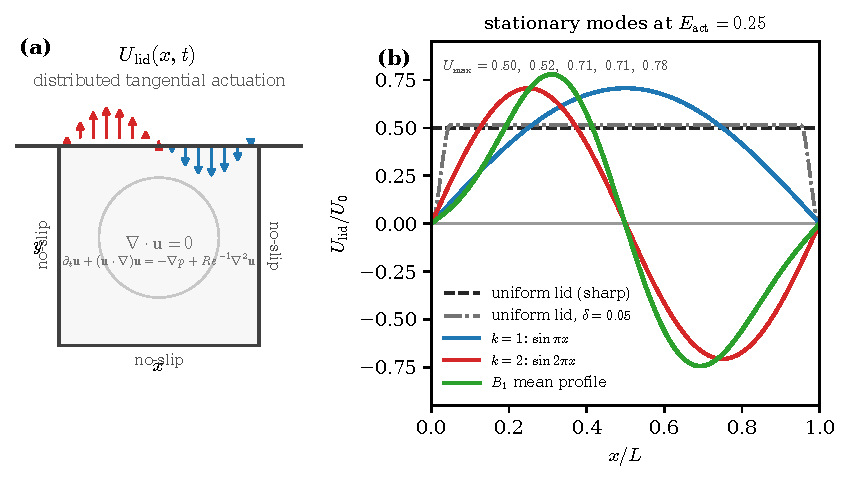
\includegraphics[width=\textwidth]{figures/fig01_modes.pdf}
\caption{(a) Geometry of the controlled cavity. The upper wall moves tangentially
with a distributed profile $U_{\mathrm{lid}}(x,t)$; the three other walls are
no-slip and stationary. (b) The five stationary actuation profiles compared in
this study, all normalized to the same quadratic actuation norm
$E^\ast=\int_0^1U_{\mathrm{lid}}^2\,dx=0.25$. The maximum wall velocity differs
between profiles at equal norm: $U_{\max}=0.50$ for the uniform lid, $0.71$ for
the two harmonics and $0.78$ for the $B_1$ mean profile.}
\label{fig:modes}
\end{figure}

\subsection{Identified actuation branches}
\label{sec:branches}

The time-dependent actuations are three representatives identified by the
physics-informed procedure of Sec.~\ref{sec:methods} and classified by the modal
energy of their control coefficients (details of the identification campaign and
classification rules are provided in supplementary Tables~S1--S3 and Fig.~S3). Writing the lid as
\begin{equation}
U_{\mathrm{lid}}(x,t)=\sum_{m=1}^{N_x}\sum_{n=0}^{N_t-1}
a_{mn}\sin(m\pi x)\cos(n\pi t),
\label{eq:fourier}
\end{equation}
the energy of coefficient $(m,n)$ is $\mathcal{E}_{m0}=\tfrac12a_{m0}^2$ and
$\mathcal{E}_{mn}=\tfrac14a_{mn}^2$ for $n\ge1$, with normalized fractions
$f_{mn}=\mathcal{E}_{mn}/\sum\mathcal{E}_{ij}$. The stationary second-harmonic
fraction is $f_2\equiv f_{20}$ and the total time-dependent fraction is
$f_t=\sum_{n\ge1}f_{mn}$. The three classes are defined by modal dominance
\cite{beniaiche2026}: $B_1$ has $f_2>2f_t$ and $f_2>0.5$ (stationary
second-harmonic dominated); $B_2$ has $f_t>2f_2$ and $f_t>0.5$ (temporally
dominated); $B_3$ satisfies neither condition (mixed). At $Re=500$ and
$E^\ast=0.25$ the representatives used here have
$(f_2,f_t)=(0.93,0.07)$ for $B_1$, $(0.00,1.00)$ for $B_2$ (seed 5) and
$(0.52,0.45)$ for $B_3$ (seed 0), with a first-harmonic content
$f_1=0.006$ for $B_3$ and below $0.02$ for the other two.

The $B_1$ representative is used in two forms. The \emph{full} series is the
control as identified, including its small temporal content; the \emph{mean
profile} is its time average, a stationary actuation that isolates the spatial
structure. The stationary comparison of Sec.~\ref{sec:stationary} uses the mean
profile and the cycle-mean comparison of Sec.~\ref{sec:branches} uses the full
series, so that the effect of the spatial structure is never conflated with the
effect of the temporal one. Representative profiles and their space--time
structure are shown in Fig.~\ref{fig:signatures}; Table~\ref{tab:modes}
collects the characteristics of the eight actuations compared in the paper.

\begin{figure}[t]
\centering
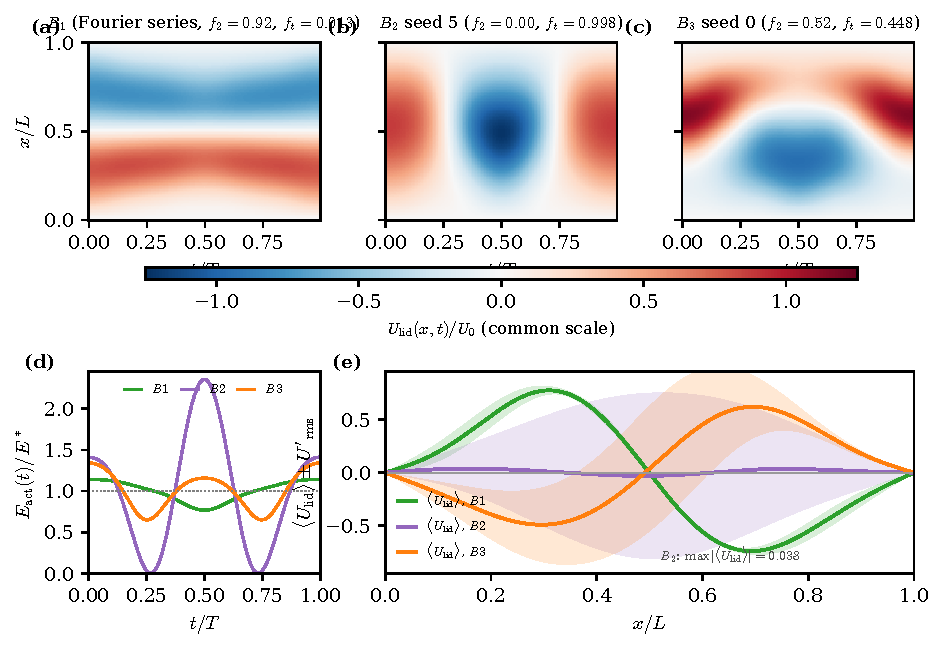
\includegraphics[width=\textwidth]{figures/fig02_signatures.pdf}
\caption{Spatio-temporal structure of the three identified branch controls at
$Re=500$ and $\overline{E}_{\mathrm{act}}=0.25$. (a)--(c) Lid velocity
$U_{\mathrm{lid}}(x,t)$ over one forcing period, on a common colour scale.
$B_1$ is nearly stationary; $B_2$ oscillates with a full sign reversal, the wall
velocity vanishing twice per period; $B_3$ combines a stationary two-lobe pattern
with a strong oscillation. (d) Instantaneous actuation norm $\Eact(t)$ normalized
by the common cycle-mean target: $B_2$ spans $0.004$--$2.36\,E^\ast$, whereas
$B_1$ stays within $0.77$--$1.14\,E^\ast$ and $B_3$ within $0.65$--$1.34\,E^\ast$.
The comparison is therefore made at equal \emph{cycle-mean} norm, not at equal
instantaneous norm. (e) Time-mean lid profile with the temporal standard
deviation as a band; the $B_2$ mean profile reaches only $0.039$, so a mean-field
diagnostic sees almost no actuation.}
\label{fig:signatures}
\end{figure}

\begin{table}[t]
\centering
\caption{Actuation modes and hydrodynamic states compared in this study
($Re=500$, fixed viscosity and geometry). $U_{\max}$ is the maximum of the
time-mean lid profile and $Re_{\max}=U_{\max}Re$ the corresponding effective
Reynolds number; for the two time-dependent branches the maximum over the whole
period is given in parentheses. All stationary profiles and the cycle means of
the time-dependent ones carry the same quadratic actuation norm,
$\overline{E}_{\mathrm{act}}=0.25$; the instantaneous norm of $B_2$ and $B_3$
varies over the period. $f_2$ and $f_t$ are the stationary second-harmonic and
total temporal energy fractions of the control coefficients.}
\label{tab:modes}
\footnotesize
\setlength{\tabcolsep}{4pt}
\begin{tabular}{llccccc}
\toprule
Actuation & Structure & $U_{\max}$ & $Re_{\max}$ & $f_2$ & $f_t$ & Role\\
\midrule
Uniform lid & constant, sharp corners & 0.50 & 250 & --- & 0 & reference\\
Uniform lid, $\delta=0.05$ & constant, tapered & 0.52 & 258 & --- & 0 & converged ref.\\
$k=1$ & $\sin\pi x$ & 0.71 & 354 & 1.00 & 0 & control\\
$k=2$ & $\sin 2\pi x$ & 0.71 & 354 & 1.00 & 0 & control\\
$B_1$ mean profile & mean of $B_1$ & 0.78 & 390 & 0.93 & 0 & stationary\\
$B_1$ full series & Fourier series & 0.78 (0.82) & 388 & 0.93 & 0.07 & branch\\
$B_2$ seed 5 & temporal & 0.04 (1.23) & 20 & 0.00 & 1.00 & unsteady\\
$B_3$ seed 0 & mixed & 0.62 (1.16) & 311 & 0.52 & 0.45 & intermediate\\
\bottomrule
\end{tabular}
\end{table}

%----------------------------------------------------------------------
\section{Numerical methodology}
\label{sec:methods}
%----------------------------------------------------------------------

\subsection{Identification of the actuation}

The control coefficients $a_{mn}(Re)$ and the flow field are obtained simultaneously
by a parametric physics-informed neural network with inputs $(x,y,t,\widetilde{Re})$
and a multi-objective loss combining the momentum and continuity residuals, the
boundary conditions, a viscous-dissipation objective, the actuation-norm
constraint $(\Eact-E^\ast)^2$, a spatial-variance regularizer and a
Reynolds-separation term. The identification is performed once over
$Re\in[100,1000]$; the branch representatives at $Re=500$, $E^\ast=0.25$ are then
exported on one forcing period and transferred without retraining. The network
architecture, the sampling protocol, the loss weights, the training schedule and
the branch-classification rules are reported in the Supplementary Material
(Secs.~S1--S2) and in Ref.~\cite{beniaiche2026}; the present paper uses the
identified controls as physical boundary data and does not re-examine the
identification procedure. What matters here is only that the exported profile is
the one the optimizer produced, without harmonic substitution or spatial
idealization, and that its realized norm is the prescribed one to within
$0.16\%$.

\subsection{Independent MRT-LBM evaluation}

The flows are computed with a multiple-relaxation-time D2Q9 lattice-Boltzmann
solver \cite{dhumieres2002mrt,chen1998doolen} that is independent of the
identification framework: a Cartesian lattice instead of scattered collocation, a
different discretization of the same equations, and a different iteration
strategy. Collision is performed in moment space with a diagonal relaxation
matrix, and the moving lid is imposed with the Zou--He velocity boundary
condition \cite{zou1997pressure,pan2006high}. The solver reproduces the benchmark
centerline velocities of Ghia et al.~\cite{ghia1982high} with
$L_2(u)=0.0051$ and $L_\infty(u)=0.0128$ at $Re=100$, and
$L_2(u)=0.0141$ and $L_\infty(u)=0.0300$ at $Re=1000$ on the
$256\times256$ lattice (Supplementary Table~S1), which fixes the resolution used
for the controlled flows.

Each actuation is advanced from rest with the lid switched on at $t=0$. At least
200 forced periods are discarded, a drift test on the cycle-averaged dissipation
fixes the end of the settling phase, and 64 consecutive periods are retained for
the statistics. The same protocol is used for every case, so the comparison does
not depend on the transient length. Instantaneous dissipation, kinetic energy and
lid power are accumulated at every step; the cycle mean is a direct accumulation
over the 64 sampled periods, not an eight-point phase quadrature, because the
latter is $5\%$ low for the most unsteady responses. The wall shear in
Eq.~\eqref{eq:plid} is evaluated with a first-order one-sided derivative of the
recovered wall velocity, and the resulting estimator uncertainty is quantified in
Sec.~\ref{sec:budget}.

\subsection{Grid convergence and uncertainty}

The three stationary controls and both uniform references are computed on
$N=128$, $256$ and $512$ lattices. The observed order of convergence
$p_{\mathrm{obs}}$ and the fine-grid grid-convergence index are obtained by
Richardson extrapolation with a safety factor $F_s=1.25$
\cite{roache1994perspective,celik2008procedure}. A triple is flagged, and its
extrapolated value discarded, when it is non-monotone, when
$p_{\mathrm{obs}}\notin[0.1,4]$, or when the GCI exceeds $100\%$: in those cases
the smooth-error assumption underlying the estimator is not credible. The
estimator is applied both to the absolute dissipation and to the dissipation
ratios, since the ratios are the quantities used in the physical discussion and
their errors need not cancel. The time-dependent branches are ranked on a single
$N=256$ lattice, with two realizations per branch; that restriction is stated
wherever those numbers are used.

%----------------------------------------------------------------------
\section{Energetic response of stationary wall-actuation modes}
\label{sec:stationary}
%----------------------------------------------------------------------

\subsection{Comparison at matched actuation norm}

Table~\ref{tab:stationary} and Fig.~\ref{fig:gci} give the integrated dissipation
of the five stationary controls at $Re=500$ and $E^\ast=0.25$. On the finest grid
the first harmonic is the only control that lowers the dissipation relative to the
uniform lid of the problem statement: $\varepsilon_{512}=0.00713$ against
$0.01102$, a ratio of $0.647$. The second harmonic raises it to $0.01185$
(ratio $1.076$) and the $B_1$ mean profile to $0.01250$ (ratio $1.134$). The
ordering $k=1<\text{uniform}<k=2\approx B_1$ is the central stationary result, and
it is the reverse of the fixed-lid-velocity ordering reported in
Ref.~\cite{beniaiche2026}, where both harmonic profiles were less dissipative than
the uniform lid and the second harmonic was the least dissipative of the three.
The reversal is not a refinement of that result but a consequence of the
constraint: at equal lid speed the harmonics have half the norm of the uniform
lid, and restoring the norm raises their wall velocity by $\sqrt2$ and their
effective Reynolds number with it.

\begin{table}[t]
\centering
\caption{Stationary controls at $Re=500$ and matched quadratic actuation norm
$E^\ast=0.25$ on three grids. $\varepsilon_N$ is the integrated viscous
dissipation; $p_{\mathrm{obs}}$ and $\mathrm{GCI}_{512}$ are the observed order
and the fine-grid grid-convergence index of the absolute dissipation
($F_s=1.25$). The last column gives the dissipation normalized by the sharp
and by the corner-regularized uniform lid on the same grid (the two values are
separated by a slash). The $B_1$ mean profile
is used as computed ($E_r=0.2503$). A dagger marks a flagged triple, for which
the extrapolated value is not used. $U_{\max}$ and $Re_{\max}$ are repeated here
because the norm constraint fixes the rms wall velocity ($0.5$) but not the peak.}
\label{tab:stationary}
\footnotesize
\setlength{\tabcolsep}{4pt}
\begin{tabular}{lcccccccc}
\toprule
Control & $U_{\max}$ & $Re_{\max}$ & $\varepsilon_{128}$ & $\varepsilon_{256}$ & $\varepsilon_{512}$
& $p_{\mathrm{obs}}$ & GCI$_{512}$ (\%) & $\varepsilon_{512}/\varepsilon^{\mathrm{ref}}_{512}$ (sharp / reg.)\\
\midrule
Uniform lid (sharp) & 0.50 & 250 & 0.00774 & 0.00948 & 0.01102 & 0.18 & 130.71$^{\dagger}$ & 1.000 / 1.272\\
Uniform lid, $\delta=0.05$ & 0.52 & 258 & 0.00717 & 0.00815 & 0.00866 & 0.96 & 7.79 & 0.786 / 1.000\\
$k=1$ ($\sin\pi x$) & 0.71 & 354 & 0.00635 & 0.00688 & 0.00713 & 1.09 & 3.85 & 0.647 / 0.823\\
$k=2$ ($\sin 2\pi x$) & 0.71 & 354 & 0.01012 & 0.01129 & 0.01185 & 1.04 & 5.62 & 1.076 / 1.368\\
$B_1$ mean profile & 0.78 & 390 & 0.01067 & 0.01189 & 0.01250 & 1.01 & 6.01 & 1.134 / 1.443\\
\bottomrule
\end{tabular}
\end{table}

The ratios built on the sharp uniform lid are not converged estimates of the shape
effect, because the reference itself does not converge: its increments between
successive grids decay by only $12\%$ per refinement ($p_{\mathrm{obs}}=0.18$,
GCI $131\%$), and the formal Richardson limit, $2.25\times10^{-2}$, is more than
twice the finest-grid value and is not a credible continuous-limit dissipation.
The three other controls converge, with $p_{\mathrm{obs}}=1.09$, $1.04$ and
$1.01$ and fine-grid GCIs of $3.9\%$, $5.6\%$ and $6.0\%$. Normalizing by the
corner-regularized lid instead gives ratios of $0.823$, $1.368$ and $1.443$ at
$N=512$, i.e.\ $-17.7\%$, $+36.8\%$ and $+44.3\%$, with Richardson estimates
$0.802$, $1.347$ and $1.427$ and ratio GCIs of $3.1\%$, $1.9\%$ and $1.4\%$. The
sign of the ordering is the same under both references and at all three
resolutions; only its magnitude changes, because the non-converged corner
contribution inflates the denominator of the sharp-lid ratios. We therefore quote
the regularized ratios as the better-defined estimate of the shape effect and the
sharp-lid ratios as the values directly comparable with the classical uniform-lid
baseline, and we do not use the sharp-lid ratio for $k=1$ as a quantitative
reduction: $-35.3\%$ overstates the $-17.7\%$ obtained against a converged
reference. The separation between $k=2$ and the $B_1$ mean profile
($1.368$ against $1.443$, about $5\%$) exceeds their GCIs but not by a wide
margin, so they are reported as approximately equal rather than strictly ordered.

\begin{figure}[t]
\centering
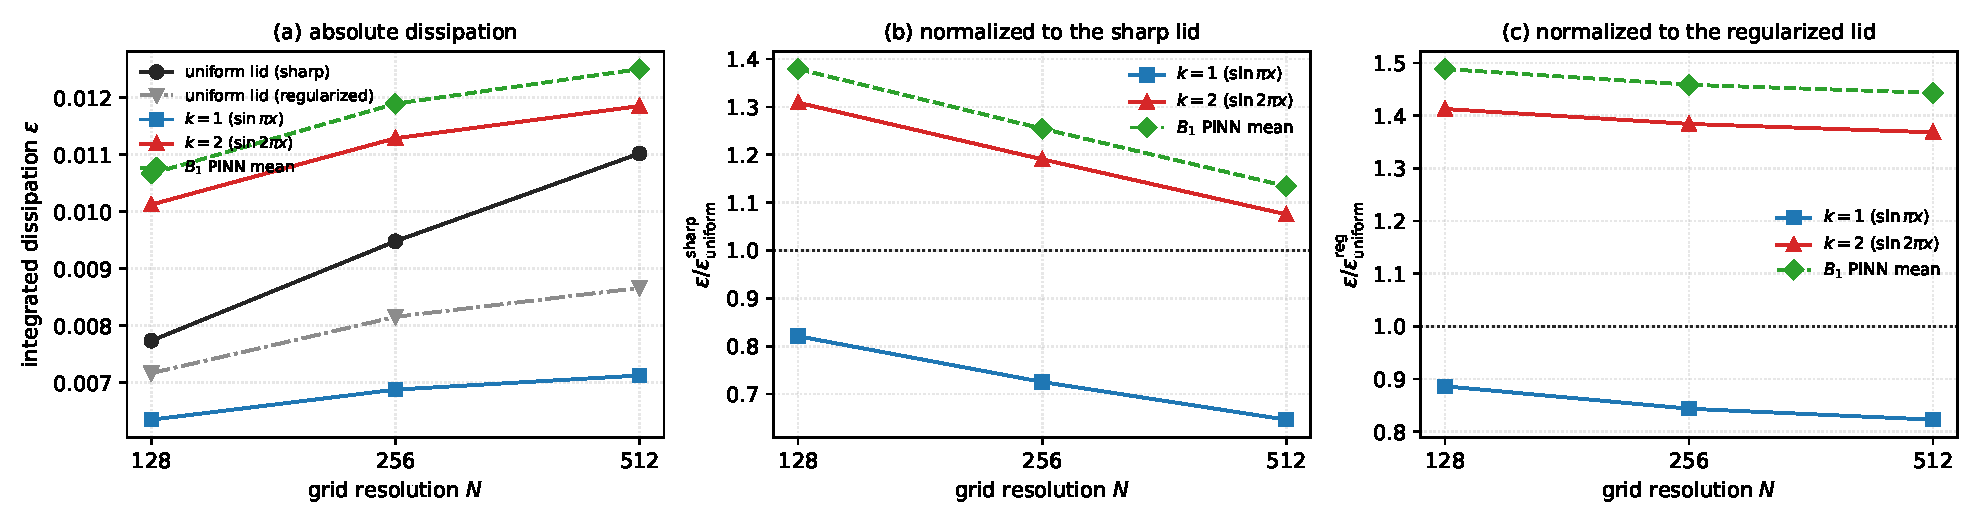
\includegraphics[width=0.92\textwidth]{figures/fig12_gci_updated.pdf}
\caption{Grid convergence of the stationary comparison at $Re=500$ and matched
actuation norm $E^\ast=0.25$. (a) Integrated dissipation versus resolution for the
four stationary controls and for the corner-regularized uniform lid. (b)
Dissipation normalized by the sharp uniform lid on the same grid: this reference
does not converge, and the ratios drift by $18$--$21\%$ over the triple. (c)
Dissipation normalized by the regularized lid: the three ratio triples are
monotone and converge with GCIs of $1.4$--$3.1\%$. The sign of the ordering
$k=1<\text{uniform}<k=2\approx B_1$ is observed at every resolution in both (b)
and (c); its magnitude is reference-dependent.}
\label{fig:gci}
\end{figure}

\subsection{The corner singularity and the reference dependence}
\label{sec:corner}

The non-convergence of the uniform lid is a property of its corners, not of the
uniform profile as such. Its dissipation grows by $16\%$ between $N=256$ and
$N=512$, the signature of a boundary-layer singularity that the grid cannot
resolve. Replacing the discontinuity by the cosine taper of Eq.~\eqref{eq:taper}
removes $21\%$ of the dissipation at $N=512$ and, more importantly, changes the
growth between the two finest grids from $16\%$ to $6\%$, i.e.\ the expected
first-order rate: $p_{\mathrm{obs}}=0.96$, GCI $7.8\%$, extrapolated
$\varepsilon_\infty=9.20\times10^{-3}$. A continuous lid therefore converges, and
the singular one does not. This has two consequences for the interpretation. First,
a comparison of actuation shapes that uses the discontinuous lid as denominator
mixes the shape effect with a resolution artefact; the regularized reference is
the only one that separates them. Second, the corner is an energetic feature in
its own right: the uniform lid concentrates a large part of its dissipation in two
small regions whose contribution grows with resolution, so any ranking that
depends on the corner peak is resolution-dependent by construction.

The practical conclusion is that two numbers must be reported for each profile,
not one. The sharp-lid ratio answers the question ``what does this actuation do
relative to the classical cavity?'' and is the quantity a reader will compare with
the literature. The regularized ratio answers ``what is the effect of the spatial
shape at fixed actuation norm?'' and is the quantity that supports a physical
statement about shape. Both are given in Table~\ref{tab:stationary}, and the text
uses the second for every claim about ordering or magnitude.

\subsection{Local mechanism of the second-harmonic penalty}
\label{sec:mechanism}

The ranking has a local origin that can be read directly from the fields
(Fig.~\ref{fig:mechanism}). The uniform lid concentrates its dissipation in the
two upper corners, where the imposed tangential velocity jumps to zero: the peak
strain-rate magnitude there is $169$ in units of $U_0/L$, against $15.0$ for
$k=1$ and $23.4$ for $k=2$, and those corner layers are the brightest features of
the dissipation field. Both harmonics remove the jump, and their dissipation is
spread over the lid shear layer and the side walls instead. But the second
harmonic pays for this in the interior. Its lid generates a pair of
counter-rotating cells of nearly equal strength, separated by a wall-to-wall
separatrix at $x=0.5$, each enclosing its own low-strain core; the uniform and
first-harmonic lids recover the classical single primary vortex with a corner
eddy. The reorganization shifts the strain-rate distribution towards larger
values: the interior mean $\langle|\Sij|\rangle$ is $1.450$ for $k=2$, against
$1.039$ for the uniform lid and $1.088$ for $k=1$, a $40\%$ increase at identical
actuation norm.

The trade-off is explicit. The first harmonic removes almost all of the corner
peak ($169$ to $15.0$) at a cost of $4.7\%$ in interior mean strain, and is a net
reduction. The second harmonic removes slightly less of it ($23.4$) while raising
the interior mean by $39.6\%$, and is a net penalty: it buys a symmetric two-cell
state with a stronger interior strain field, and the corner singularity it removes
is not costly enough to compensate. The second harmonic therefore pays roughly
$40\%$ more interior strain to avoid a corner peak that contributes less than
$5\%$ of the total dissipation. Additional parametric studies (network capacity,
loss-term ablation, aspect-ratio dependence, and Fourier vs.\ Chebyshev bases)
are reported in supplementary Secs.~S3--S7 and Figs.~S5--S7; they confirm that
the ordering is robust to the numerical parameters and is a physical property of
the flow response to the actuation structure.
eight times the interior penalty of the first for no additional corner gain. This
is the mechanical content of the $+36.8\%$ and $+44.3\%$ of
Table~\ref{tab:stationary}: the energetic cost of a spatial mode is set by the
volume over which it raises the strain, not by the peak it removes.

\begin{figure}[t]
\centering
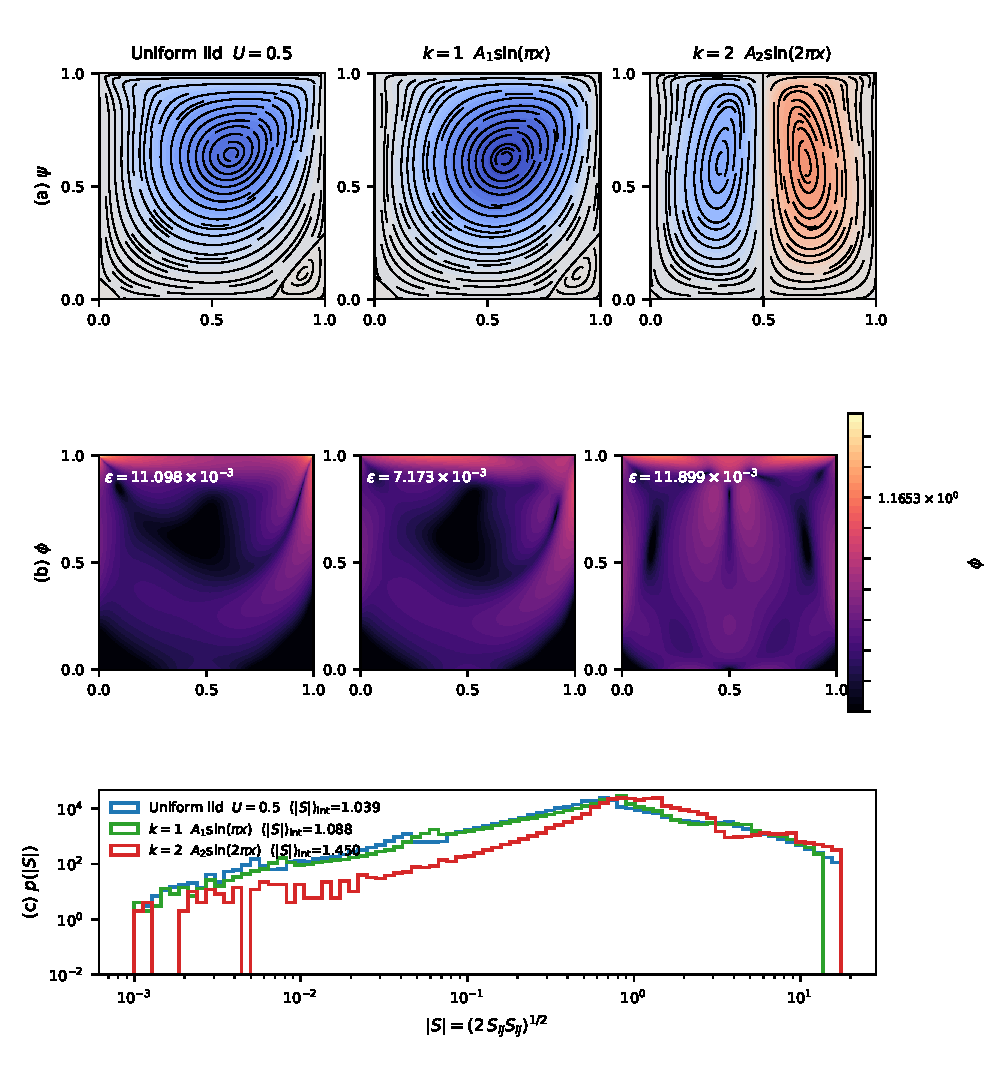
\includegraphics[width=0.78\textwidth]{figures/fig15_mechanism_iso.pdf}
\caption{Local origin of the stationary ranking at $Re=500$, $N=512$ and matched
actuation norm, on scales common to the three columns. (a) Stream function of the
steady response with the streamline topology. (b) Local viscous dissipation
$\phi=\nu(2S_{11}^2+2S_{22}^2+4S_{12}^2)$ on a logarithmic scale spanning six
decades below the global maximum; the annotation gives the domain integral. (c)
Probability density of the strain-rate magnitude over the cavity interior (three
boundary cells excluded), with the interior mean
$\langle|\Sij|\rangle_{\mathrm{int}}$. The uniform lid peaks at the corners
($|\Sij|_{\max}=169$); $k=1$ removes the peak at almost no interior cost
($\langle|\Sij|\rangle_{\mathrm{int}}=1.088$ against $1.039$); $k=2$ removes less
of it ($23.4$) and raises the interior mean to $1.450$, which is the origin of
its dissipation penalty.}
\label{fig:mechanism}
\end{figure}

%----------------------------------------------------------------------
\section{Cycle-mean dissipation of time-dependent actuation branches}
\label{sec:branches_results}
%----------------------------------------------------------------------

\subsection{Why the dissipation of the mean flow is not the cycle mean}

For the stationary controls of Sec.~\ref{sec:stationary} the distinction between
$D(\overline{\mathbf{u}})$ and $\Dbar$ is empty, because the response is steady.
For the time-dependent branches it becomes the central issue. Equation
\eqref{eq:jensen} is exact: the cycle mean exceeds the mean-field value by the
dissipation of the fluctuations, and there is no reason for that term to be small
when the actuation reverses sign. A mean-field diagnostic answers the question
``how much would this flow dissipate if it were steady?''; it does not answer
``how much does it dissipate?''. Figure~\ref{fig:cycle} and
Table~\ref{tab:cycle} show how far apart the two answers can be; supplementary
Table~S5 and Fig.~S8 provide additional temporal statistics and phase-resolved
analyses for the three branches.

\begin{figure}[t]
\centering
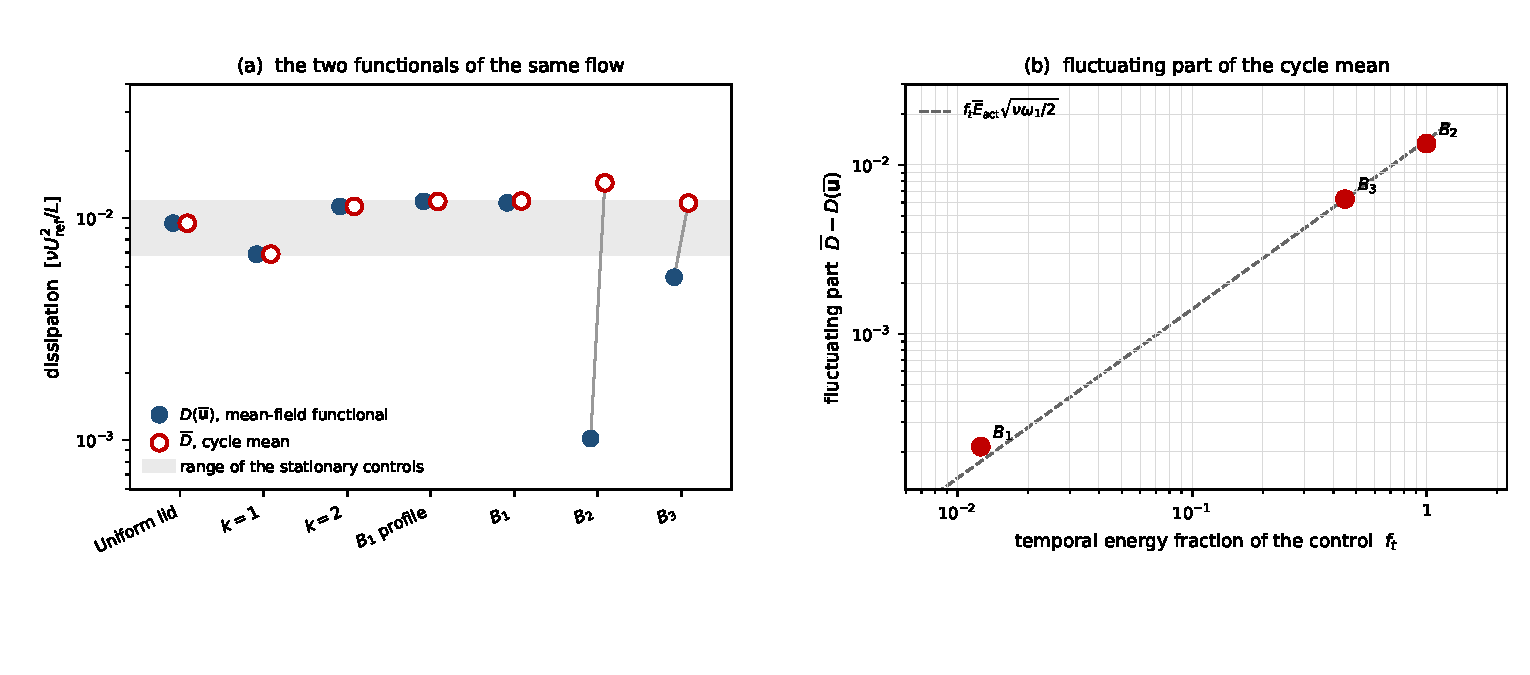
\includegraphics[width=0.94\textwidth]{figures/fig18_branch_iso_cycle.pdf}
\caption{Iso-energetic comparison of the nine controls at $Re=500$,
$\overline{E}_{\mathrm{act}}=0.25$ and $N=256$. Left: the two dissipation
functionals of each control, the dissipation of the time-mean field (filled
markers) and the cycle mean (open markers), joined by the gap between them; the
two coincide for stationary controls. Right: cycle-mean dissipation against the
temporal energy fraction $f_t$ of the lid control. The ordering in $f_t$ is the
order in which the branches are recovered by the identification, and it is not the
order of the dissipation cost.}
\label{fig:cycle}
\end{figure}

\subsection{Cycle-mean comparison of the three branches}
\label{sec:branch_compare}

Table~\ref{tab:cycle} collects the result. The five quasi-stationary controls span
less than a factor of two, from $6.88\times10^{-3}$ for $k=1$ to
$1.22\times10^{-2}$ for the full $B_1$ series, and their mean-field and cycle-mean
values coincide to within $4\%$; for the $B_1$ series the difference is
$1.17\times10^{-2}$ against $1.22\times10^{-2}$, which is the residual effect of
its small temporal content. The branches with substantial temporal content leave
that band. $B_2$ dissipates $3.76\times10^{-2}$ over the cycle while its mean
field dissipates $3.10\times10^{-5}$, a ratio of $1214$; its mean field holds only
$6\%$ of the cycle-mean kinetic energy, so the mean motion is a shallow
recirculation under the lid, not a weakened copy of the instantaneous flow. $B_3$
is intermediate: $D(\overline{\mathbf{u}})=5.05\times10^{-3}$ and
$\Dbar=2.18\times10^{-2}$, a ratio of $4.3$. On the cycle average, and at the same
actuation norm, $B_2$ costs $3.1$ times $B_1$ and $5.5$ times the least
dissipative stationary control; its two realizations agree to $1.7\%$, whereas the
two $B_3$ realizations differ by $23\%$, so the $B_3$ value quoted here is the
lower of the two and must be read as a lower bound on that class.

\begin{table}[t]
\centering
\caption{Dissipation of the time-mean field and cycle-mean dissipation at
$Re=500$, $N=256$ and cycle-mean actuation norm $\overline{E}_{\mathrm{act}}=0.25$.
$D(\overline{\mathbf{u}})$ is the functional evaluated on the time-mean field;
$\Dbar$ is the average of the instantaneous dissipation over the phase-resolved
periodic response and is the performance index relevant to a periodic flow. The
two coincide only in the steady limit. $A_\varepsilon$ is the half-spread of
$D(t)$ over the cycle, i.e.\ the variability concealed by a single cycle-mean
number. The $B_1$ mean profile row is stationary by construction; the $B_1$ full
row is the identified series.}
\label{tab:cycle}
\small
\begin{tabular}{lcccccc}
\toprule
Control & $f_t$ & $\overline{E}_{\mathrm{act}}$ & $D(\overline{\mathbf{u}})$ & $\Dbar$
& $\Dbar/D(\overline{\mathbf{u}})$ & $A_\varepsilon$\\
\midrule
Uniform lid & 0.000 & 0.250 & $9.48\times10^{-3}$ & $9.48\times10^{-3}$ & 1.00 & $0$\\
$k=1$ ($\sin\pi x$) & 0.000 & 0.250 & $6.88\times10^{-3}$ & $6.88\times10^{-3}$ & 1.00 & $0$\\
$k=2$ ($\sin 2\pi x$) & 0.000 & 0.250 & $1.13\times10^{-2}$ & $1.13\times10^{-2}$ & 1.00 & $0$\\
$B_1$ mean profile & 0.000 & 0.250 & $1.19\times10^{-2}$ & $1.19\times10^{-2}$ & 1.00 & $0$\\
$B_1$ full series & 0.074 & 0.250 & $1.17\times10^{-2}$ & $1.22\times10^{-2}$ & 1.04 & $2.4\times10^{-3}$\\
$B_2$ seed 5 & 0.998 & 0.250 & $3.10\times10^{-5}$ & $3.76\times10^{-2}$ & 1214 & $3.6\times10^{-2}$\\
$B_2$ seed 14 & 0.975 & 0.250 & $1.82\times10^{-4}$ & $3.70\times10^{-2}$ & 204 & $3.5\times10^{-2}$\\
$B_3$ seed 0 & 0.448 & 0.250 & $5.05\times10^{-3}$ & $2.18\times10^{-2}$ & 4.3 & $1.5\times10^{-2}$\\
$B_3$ seed 4 & 0.637 & 0.250 & $3.12\times10^{-3}$ & $2.69\times10^{-2}$ & 8.6 & $2.6\times10^{-2}$\\
\bottomrule
\end{tabular}
\end{table}

Three statements follow, and they are the ones the paper retains. First, the
mean-field functional is not a surrogate for the cycle mean: it can be three
orders of magnitude too small and it reverses the ranking of the branches. Second,
the temporal fraction $f_t$ orders the branches by accessibility, not by cost:
$B_2$, the most strongly time-dependent control, is the most dissipative of the
three at matched norm. Third, the ranking of the time-dependent branches
($B_1<B_3<B_2$) is the same as the ranking of their mean-field dissipation read in
reverse, which is a direct consequence of Eq.~\eqref{eq:jensen}: the branch that
suppresses its mean flow most effectively is the one that pays most in
fluctuations.

\subsection{Flow organization behind the cycle-mean cost}
\label{sec:topology}

The field-level organization explains the numbers (Figs.~\ref{fig:topology}
and~\ref{fig:velocity}). The $B_1$ time-mean flow is the familiar pair of
counter-rotating cells centred at $(0.31,0.54)$ and $(0.69,0.56)$, with
$\max|\langle\mathbf{u}\rangle|=0.733$ and $\langle\psi\rangle\in[-0.036,0.035]$;
half of its mean kinetic energy lies below $y=0.675$, so the cells fill the
cavity. Its instantaneous states coincide with that mean to $2.7\%$ in field norm
and its kinetic-energy fluctuation ratio is $R_K=4\times10^{-4}$, so it is
quasi-stationary in the operational sense. The $B_2$ mean field is $19$ times
weaker in stream function ($\max|\langle\psi\rangle|=0.0019$) and $18$ times weaker
in peak speed ($0.042$, or $5.7\%$ of the $B_1$ value); its mean extrema sit at
$y=0.89$--$0.92$ and half of the mean kinetic energy lies above $y=0.95$. Its
streamwise fluctuation, by contrast, reaches $0.555$---thirteen times its own mean
and $76\%$ of the $B_1$ mean peak. The $B_3$ flow keeps an intermediate mean
circulation ($\max|\langle\mathbf{u}\rangle|=0.595$, $81\%$ of $B_1$) but places
it close to the lid, with extrema at $(0.20,0.86)$ and $(0.77,0.81)$ and half of
the mean kinetic energy above $y=0.91$; its fluctuation reaches $0.416$.

``Weak mean flow'' is therefore not ``weak flow''. The controls with a strong
temporal component do not produce a small perturbation around a mean
recirculation: they produce responses whose fluctuations dominate the
instantaneous field while the mean is nearly zero. A figure that normalized each
panel by its own maximum, or a diagnostic that used only the mean field, would
hide exactly the contrast that defines the two unsteady branches.

\begin{figure}[t]
\centering
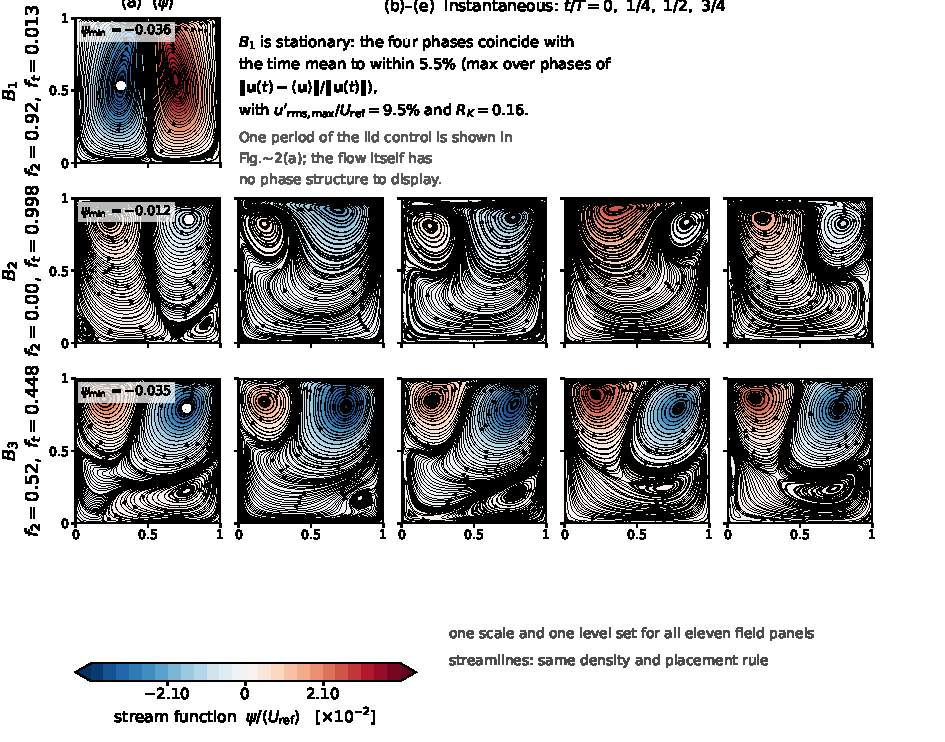
\includegraphics[width=\textwidth]{figures/fig20_branch_topology.pdf}
\caption{Flow topology of the three branch controls at $Re=500$,
$E^\ast=0.25$ and $N=256$, on one stream-function scale and one set of contour
levels common to all panels. Rows: $B_1$ (full series, $f_t=0.074$), $B_2$
(seed 5, $f_t=0.998$) and $B_3$ (seed 0, $f_2=0.520$, $f_t=0.448$). (a) Time mean
$\langle\psi\rangle$ with the streamlines of the mean flow; the circle marks its
negative extremum. (b)--(e) Instantaneous $\psi$ and streamlines at
$t/T=0,1/4,1/2,3/4$ for $B_2$ and $B_3$; the four phases belong to the same
periodic state, whose first- and second-half phase averages differ by at most
$1.0\times10^{-3}$ in relative field norm. For $B_1$ the instantaneous states
coincide with the mean to $2.7\%$, so the four panels are replaced by that
statement. The common scale is deliberate: the $B_2$ mean cell is $19$ times
weaker than the $B_1$ one and is nearly invisible, which is the point.}
\label{fig:topology}
\end{figure}

\begin{figure}[t]
\centering
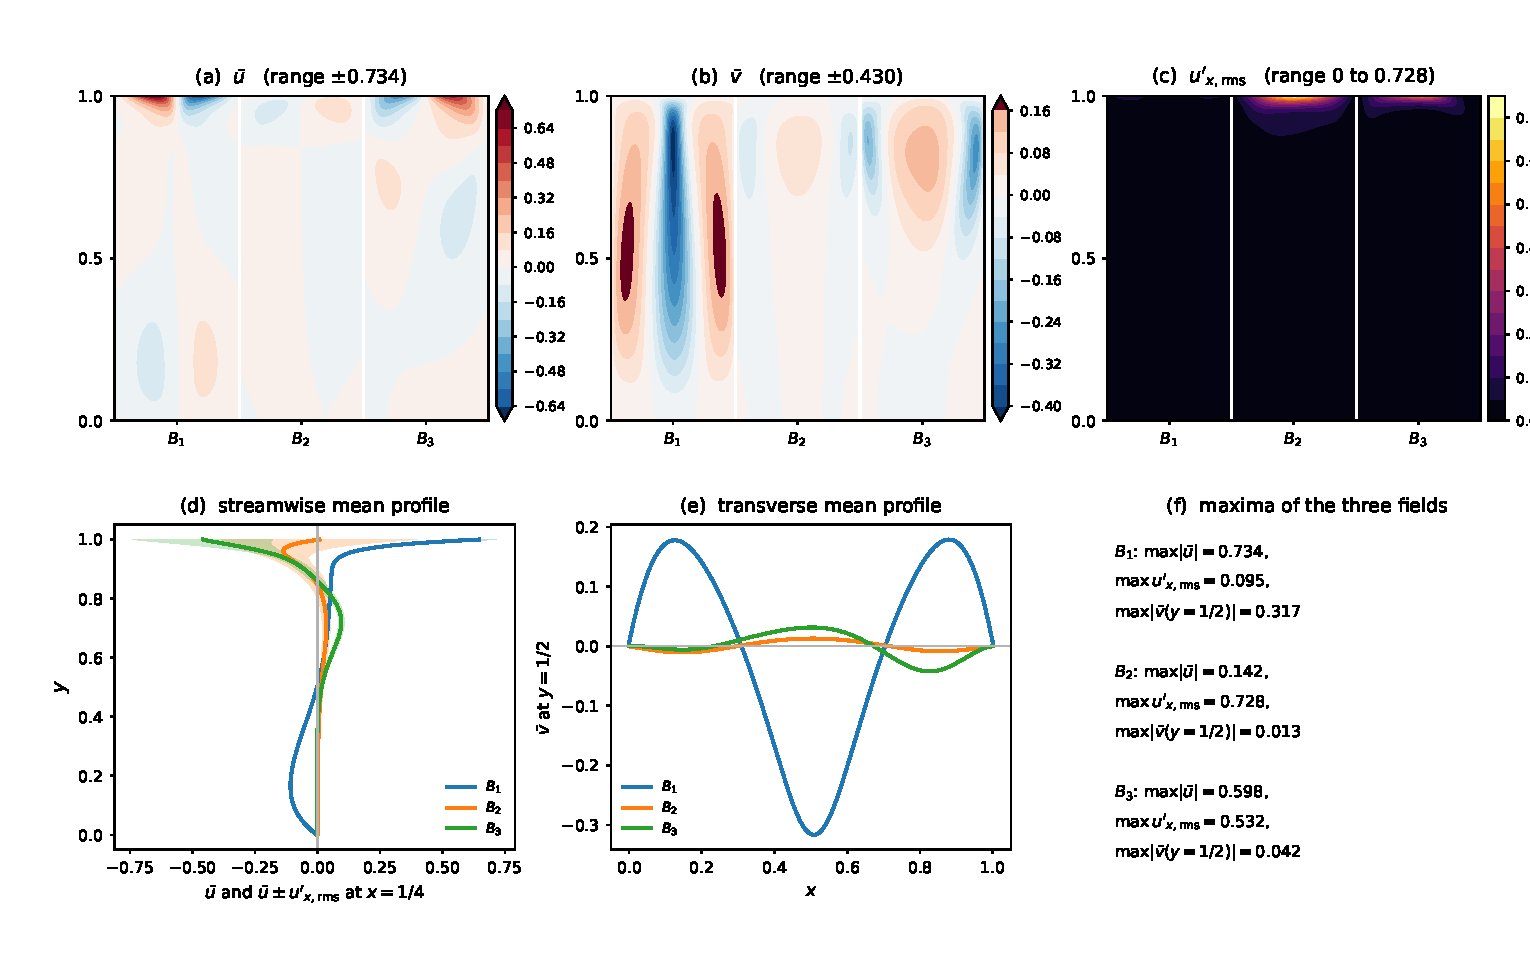
\includegraphics[width=0.92\textwidth]{figures/fig21_branch_velocity.pdf}
\caption{Velocity fields and centreline profiles of the same three captures.
Rows: (a) $\bar u$, (b) $\bar v$ and (c) $u'_{x,\mathrm{rms}}$, each on one colour
range for the three columns and a single normalization, with the occupied range
written in every panel so that the common scale can be checked. Grey lines are the
zero contours of the mean fields. (d) $\bar u$ along $x=1/4$ with the
$\pm u'_{\mathrm{rms}}$ band; the midline $x=1/2$ is not used because the
antisymmetric controls have $u\equiv0$ there. (e) $\bar v$ along $y=1/2$, with
$\bar v$ on the abscissa. The bands are temporal standard deviations over the
sixty-four sampled periods, not confidence intervals.}
\label{fig:velocity}
\end{figure}

\subsection{Mechanical energy budget of the branches}
\label{sec:budget}

Table~\ref{tab:budget} and Fig.~\ref{fig:energy} close the comparison with the
budget of Eq.~\eqref{eq:budget}. The kinetic energy separates the branches by two
orders of magnitude ($1.15\times10^{-2}$, $2.47\times10^{-4}$ and
$3.98\times10^{-3}$), while the cycle-mean dissipation orders them the other way
round ($1.22\times10^{-2}$, $3.76\times10^{-2}$ and $2.18\times10^{-2}$). Within
the period, $D(t)$ varies by a factor $1.5$, $10.9$ and $4.2$ respectively, and
the lid power of $B_2$ is negative for $14\%$ of the period: the flow returns
energy through the lid while the Stokes layer spins down. The residual
$\overline{P}_{\mathrm{lid}}-\Dbar$ is $-2.6\%$, $+5.6\%$ and $+3.8\%$.

\begin{table}[t]
\centering
\caption{Mechanical energy budget of the three branch controls at $Re=500$ and
$N=256$, at the common cycle-mean actuation norm $E^\ast=0.25$: $B_1$ is the full
series ($f_t=0.074$), $B_2$ is seed 5 ($f_t=0.998$) and $B_3$ is seed 0
($f_2=0.520$, $f_t=0.448$). All quantities are cycle averages over 64 forced
periods of the instantaneous fields; $\Dbar$ is never replaced by
$D(\overline{\mathbf{u}})$. $\sigma(\Dbar)$ is the block standard error over eight
blocks of eight cycles, expanded by $t_{7,0.975}=2.365$; it is below $0.1\%$ for
all three branches because the response is periodic to better than $10^{-3}$, so
the physically relevant uncertainty is the seed-to-seed spread ($1.7\%$ within
$B_2$, $23\%$ within $B_3$). The residual
$\overline{P}_{\mathrm{lid}}-\Dbar$ is the first-order truncation of the wall-shear
estimator, not a physical imbalance (Sec.~\ref{sec:budget}).}
\label{tab:budget}
\small
\begin{tabular}{lccccc}
\toprule
Branch & $\overline{E}_{\mathrm{act}}$ & $\overline{K}$ & $\overline{P}_{\mathrm{lid}}$
& $\Dbar$ & $\sigma(\Dbar)$\\
\midrule
$B_1$ (full series) & 0.2500 & $1.15\times10^{-2}$ & $1.19\times10^{-2}$ & $1.22\times10^{-2}$ & $<0.1\%$\\
$B_2$ (seed 5) & 0.2504 & $2.47\times10^{-4}$ & $3.97\times10^{-2}$ & $3.76\times10^{-2}$ & $<0.1\%$\\
$B_3$ (seed 0) & 0.2503 & $3.98\times10^{-3}$ & $2.26\times10^{-2}$ & $2.18\times10^{-2}$ & $<0.1\%$\\
\bottomrule
\end{tabular}
\end{table}

The residual is two to three orders of magnitude larger than the drift of $K$ over
the sampling window, which is at most $1.5\times10^{-2}\%$ of $\Dbar$; it is
therefore not a failure of periodicity. It is the truncation error of the
one-sided wall-shear estimate. Two checks bound that error. First, the first-order
estimator reproduces the independently accumulated $\Plid$ of the same fields to
$0.3\%$ for $B_1$, so it is internally consistent; the residual is a property of
the estimator, not of the accumulation. Second, replacing it by a second-order
one-sided derivative on the same fields moves the $B_1$ mean-field residual from
$-2.87\%$ to $+0.58\%$, i.e.\ it crosses zero, which shows that the estimator
uncertainty is of the order of the residual itself (a few per cent). Applied to
the branch cycle means, the same change moves the $B_1$ residual to $+1.4\%$ but
inflates the $B_2$ and $B_3$ residuals, because the three-point stencil amplifies
lattice-scale noise in the thin Stokes layer. We therefore retain the first-order
estimator for all three branches, report the residual as measured, and present
Eq.~\eqref{eq:closure} as an energetic verification with a few-per-cent estimator
uncertainty rather than as an exact closure. This is sufficient for the
conclusions drawn here, which rest on differences of a factor of three, not on
the third significant digit.

\begin{figure}[t]
\centering
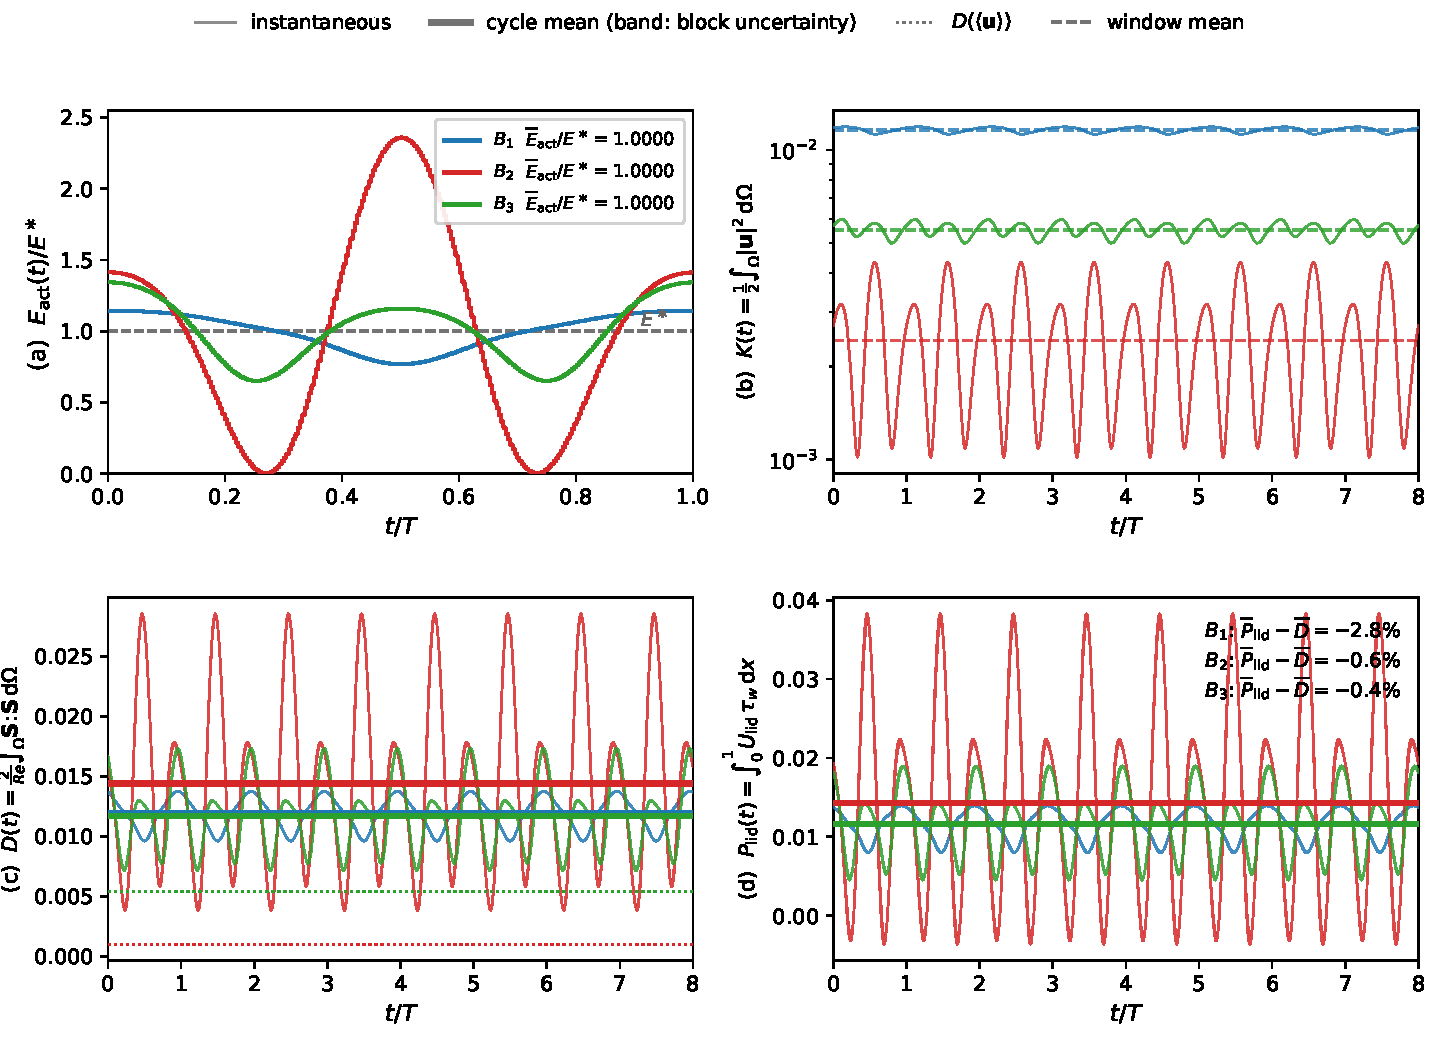
\includegraphics[width=\textwidth]{figures/fig22_branch_energy.pdf}
\caption{Phase-resolved energetic response of the three branches at $Re=500$ and
$E^\ast=0.25$. (a) Instantaneous actuation norm $\Eact(t)$ over one forced period,
normalized by the common cycle-mean target. (b) Kinetic energy $K(t)$ over the
first eight of the sixty-four sampled periods (logarithmic ordinate). (c) Viscous
dissipation $D(t)$: instantaneous (thin), cycle mean (thick, with the block
uncertainty as a band) and, dotted, the dissipation $D(\langle\mathbf{u}\rangle)$
of the time-mean field, which is not substituted for the cycle mean. (d) Lid power
$\Plid(t)$, positive into the fluid, with the same conventions; the annotations
give the window-averaged residual $\overline{P}_{\mathrm{lid}}-\Dbar$. The
kinetic-energy balance integrates to zero over one period of a periodic state, so
the two cycle means must agree; the measured residual is the wall-shear estimator
error discussed in the text.}
\label{fig:energy}
\end{figure}

%----------------------------------------------------------------------
\section{Physical interpretation and implications for flow control}
\label{sec:interpretation}
%----------------------------------------------------------------------

\subsection{Why the stationary second harmonic increases dissipation}

At matched quadratic actuation norm the second harmonic is not a low-dissipation
mode, and the reason is geometric rather than spectral. The lid profile
$A_2\sin(2\pi x)$ imposes two opposite lobes of wall velocity, which drive two
counter-rotating cells of comparable strength instead of one primary vortex. That
reorganization has two competing energetic consequences. It removes the corner
velocity jump, which suppresses a singular strain peak that dominates the
dissipation of the uniform lid. It also forces the return flow through a
wall-to-wall separatrix at the cavity centre, which raises the strain over the
whole interior: the interior mean of $|\Sij|$ increases by $40\%$ at identical
norm. The second effect wins, because the corner layer is thin while the interior
is not. The first harmonic removes the same corner peak at almost no interior
cost, and is the only stationary profile that is a net reduction. The energetic
cost of a spatial actuation mode is thus controlled by the volume over which it
raises the strain, not by the peak it removes; a mode that is ``smoother'' at the
wall need not be less dissipative in the bulk.

\subsection{Why temporal forcing increases the cycle-mean dissipation}

For a periodic control the relevant functional is the cycle mean of a quadratic
quantity, and the fluctuations are a first-order contribution to it, not a
correction. Equation~\eqref{eq:jensen} makes this explicit, and the $B_2$ branch
is its clearest illustration: a mean field that dissipates $3.1\times10^{-5}$ and
a cycle mean that dissipates $3.8\times10^{-2}$, with the mean field holding $6\%$
of the kinetic energy. The physical reason is that the oscillating lid generates a
Stokes layer whose wall-normal gradients are large and reverse twice per period;
the instantaneous strain is therefore large wherever the instantaneous velocity
is large, and the time average of its square cannot be recovered from the average
velocity. The same mechanism explains why the lid power of $B_2$ is negative for
$14\%$ of the period: while the Stokes layer spins down, the flow pushes the wall
and returns part of the energy that it received earlier. A control designer who
evaluates such a state from its mean field will conclude that it is almost
frictionless, whereas the cycle average ranks it as the most dissipative of the
three branches.

\subsection{What branch accessibility does and does not imply}

The three branches were not selected by their dissipation. They were selected by a
physics-informed optimization whose loss contains a dissipation objective, an
actuation-norm constraint and a spatial-variance regularizer, and whose outcome
depends on the initialization and on the regularization weight
\cite{beniaiche2026}. At $Re=500$ and $E^\ast=0.25$ the stationary
second-harmonic structure is the most frequently recovered one, and the full
$B_1$ series is quasi-stationary and reproducible; that is a statement about the
variational landscape, and it is confirmed here by the independent solver. It is
not a statement about efficiency. At the same actuation norm the branch most
frequently recovered is a net dissipation penalty relative to the first harmonic,
and the branch with the strongest temporal content, which is also recovered in a
reproducible way, is the most dissipative of the three. The operational
conclusion is that accessibility and physical performance are different
properties, and that a control study which reports only the recovered mode, or
only its mean-field dissipation, can invert the energetic ranking of the
actuations it compares.

Two limits of this statement must be stated explicitly, because they define its
scope. First, the temporal comparison covers three representative realizations at
a single Reynolds number ($Re=500$) and a single grid ($N=256$), with two
realizations for $B_2$ and $B_3$; the within-class spread is $1.7\%$ for $B_2$ but
$23\%$ for $B_3$, so the $B_3$ cost is a lower bound on its class. The stationary
comparison, by contrast, rests on three grids and two reference lids. Second, the
$B_1$ temporal content is small but not zero ($f_t=0.074$), and its cycle mean
exceeds its mean-field value by $4\%$; the quasi-stationary limit is approached,
not attained. Generalization to other Reynolds numbers, to three-dimensional
cavities, or to actuations with a different spatial support is not implied by the
present results.

%----------------------------------------------------------------------
\section{Conclusions}
\label{sec:conclusions}
%----------------------------------------------------------------------

Four statements summarize the study.

\begin{enumerate}
\item \emph{The spatial structure of wall actuation reorganizes the cavity and the
strain field.} At matched quadratic actuation norm the second spatial harmonic
replaces the single primary vortex of the uniform lid by two counter-rotating
cells and raises the interior mean strain rate by $40\%$; the first harmonic
removes the corner strain peak at almost no interior cost. The corner singularity
of the discontinuous lid is an energetic feature in its own right: it prevents the
convergence of the reference dissipation ($p_{\mathrm{obs}}=0.18$,
GCI $131\%$) and disappears once the corner is regularized
($p_{\mathrm{obs}}=0.96$, GCI $7.8\%$).
\item \emph{The ranking of stationary profiles depends on the constraint.} At
equal actuation norm, and relative to a converged corner-regularized reference,
the first harmonic reduces the dissipation by $17.7\%$, while the second harmonic
and the mean profile of the identified stationary branch increase it by $36.8\%$
and $44.3\%$. At equal lid speed the same three profiles are all less dissipative
than the uniform lid and the second harmonic is the best of them
\cite{beniaiche2026}; the inversion is produced by the norm constraint, which
fixes the rms wall velocity but not the peak, and therefore not the effective
Reynolds number ($Re_{\max}=250$ for the uniform lid, $354$ for the harmonics,
$390$ for the $B_1$ mean profile at $E^\ast=0.25$).
\item \emph{The cycle-mean dissipation of a time-dependent actuation is not the
dissipation of its mean field.} For the temporally dominated branch the two
differ by a factor $1214$, and the branch that is most strongly damped in the mean
is the most dissipative on the cycle ($3.76\times10^{-2}$, i.e.\ $3.1$ times the
quasi-stationary branch and $5.5$ times the first harmonic). The fluctuating part
of the strain field carries the cost, and Eq.~\eqref{eq:jensen} makes that
statement exact.
\item \emph{The branch recovered by optimization is not the branch that minimizes
dissipation at fixed control effort.} The most frequently recovered stationary
structure is a net penalty at matched norm, and the most strongly time-dependent
branch is the most dissipative of the three. Accessibility, reproducibility and
physical performance are distinct properties of an actuation, and only the last is
measured by the cycle-mean dissipation.
\end{enumerate}

The practical implication for modal flow control is that a comparison of actuation
strategies must state its constraint explicitly. Equal wall speed, equal quadratic
norm and equal mechanical power define three different problems and can produce
three different rankings; the present study uses the quadratic norm because it is
the constraint available to an optimizer, and reports the peak velocity so that
the effective Reynolds number of each comparison is visible. The cycle-mean
dissipation, not the mean-field value and not the modal spectrum, is the
performance index that follows from the energy identity.

Three extensions follow directly. A grid study of the time-dependent branches
would establish whether the factor-of-three separation is resolution-independent
to the same degree as the stationary ranking. Retraining under an explicit
cycle-mean norm constraint, rather than rescaling an identified control after the
fact, would separate the effect of the constraint from the effect of the
identification path. Finally, three-dimensional cavities would introduce spanwise
modes and test whether the two-cell second-harmonic state survives when the flow
can vary along the span. The physics-informed identification remains, in this
programme, the tool that generates the candidate actuations; the fluid-mechanical
evaluation is what decides between them.

%----------------------------------------------------------------------
\section*{Data availability}
%----------------------------------------------------------------------

The actuation series, the field captures and the post-processing scripts that
support the figures and tables of this article are available from the
corresponding author on reasonable request.

\section*{Acknowledgments}
The authors thank the Laboratory of Fluid Mechanics of the Ecole Militaire
Polytechnique for computational support.

\begin{thebibliography}{99}

\bibitem{ghia1982high}
U.~Ghia, K.~N.~Ghia, and C.~T.~Shin,
``High-Re solutions for incompressible flow using the Navier--Stokes equations and
a multigrid method,'' J.\ Comput.\ Phys.\ \textbf{48}, 387--411 (1982).

\bibitem{botella1998benchmark}
O.~Botella and R.~Peyret,
``Benchmark spectral results on the lid-driven cavity flow,''
Comput.\ Fluids \textbf{27}, 421--433 (1998).

\bibitem{shankardeshpande2000}
P.~N.~Shankar and M.~D.~Deshpande,
``Fluid mechanics in the driven cavity,''
Annu.\ Rev.\ Fluid Mech.\ \textbf{32}, 93--136 (2000).

\bibitem{albensoeder2005accurate}
S.~Albensoeder and H.~C.~Kuhlmann,
``Accurate three-dimensional lid-driven cavity flow,''
J.\ Comput.\ Phys.\ \textbf{206}, 536--558 (2005).

\bibitem{kuhlmann2019}
H.~C.~Kuhlmann and F.~Roman\`o,
``The lid-driven cavity,'' in \textit{Computational Modelling of Bifurcations and
Instabilities in Fluid Dynamics}, edited by A.~Gelfgat (Springer, Cham, 2019),
pp.~233--309.

\bibitem{gadelhak2000}
M.~Gad-el-Hak,
\textit{Flow Control: Passive, Active, and Reactive Flow Management}
(Cambridge University Press, Cambridge, 2000).

\bibitem{brunton2015closed}
S.~L.~Brunton and B.~R.~Noack,
``Closed-loop turbulence control: Progress and challenges,''
Appl.\ Mech.\ Rev.\ \textbf{67}, 050801 (2015).

\bibitem{rowley2017model}
C.~W.~Rowley and S.~T.~M.~Dawson,
``Model reduction for flow analysis and control,''
Annu.\ Rev.\ Fluid Mech.\ \textbf{49}, 387--417 (2017).

\bibitem{bewley2001dns}
T.~R.~Bewley, P.~Moin, and R.~Temam,
``DNS-based predictive control of turbulence: an optimal benchmark for feedback
algorithms,'' J.\ Fluid Mech.\ \textbf{447}, 179--225 (2001).

\bibitem{bergmann2005optimal}
M.~Bergmann, L.~Cordier, and J.-P.~Brancher,
``Optimal rotary control of the cylinder wake using proper orthogonal
decomposition reduced-order model,'' Phys.\ Fluids \textbf{17}, 097101 (2005).

\bibitem{choi1994active}
H.~Choi, P.~Moin, and J.~Kim,
``Active turbulence control for drag reduction in wall-bounded flows,''
J.\ Fluid Mech.\ \textbf{262}, 75--110 (1994).

\bibitem{quadrio2004critical}
M.~Quadrio and P.~Ricco,
``Critical assessment of turbulent drag reduction through spanwise wall
oscillations,'' J.\ Fluid Mech.\ \textbf{521}, 251--262 (2004).

\bibitem{corke2010dbd}
T.~C.~Corke, C.~L.~Enloe, and S.~P.~Wilkinson,
``Dielectric barrier discharge plasma actuators for flow control,''
Annu.\ Rev.\ Fluid Mech.\ \textbf{42}, 505--529 (2010).

\bibitem{rabsult2019drl}
J.~Rabault, M.~Kuchta, A.~Jensen, U.~R\'eglade, and N.~Cerardi,
``Artificial neural networks trained through deep reinforcement learning discover
control strategies for active flow control,''
J.\ Fluid Mech.\ \textbf{865}, 281--302 (2019).

\bibitem{garnier2021drl}
P.~Garnier, J.~Viquerat, J.~Rabault, A.~Larcher, A.~Kuhn, and E.~Hachem,
``A review on deep reinforcement learning for fluid mechanics,''
Comput.\ Fluids \textbf{225}, 104973 (2021).

\bibitem{raissi2019pinn}
M.~Raissi, P.~Perdikaris, and G.~E.~Karniadakis,
``Physics-informed neural networks: A deep learning framework for solving forward
and inverse problems involving nonlinear partial differential equations,''
J.\ Comput.\ Phys.\ \textbf{378}, 686--707 (2019).

\bibitem{cai2021pinnreview}
S.~Cai, Z.~Mao, Z.~Wang, M.~Yin, and G.~E.~Karniadakis,
``Physics-informed neural networks (PINNs) for fluid mechanics: A review,''
Acta Mech.\ Sin.\ \textbf{37}, 1727--1738 (2021).

\bibitem{noack2003hierarchy}
B.~R.~Noack, K.~Afanasiev, M.~Morzy\'nski, G.~Tadmor, and F.~Thiele,
``A hierarchy of low-dimensional models for the transient and post-transient
cylinder wake,'' J.\ Fluid Mech.\ \textbf{497}, 335--363 (2003).

\bibitem{schmid2010dmd}
P.~J.~Schmid,
``Dynamic mode decomposition of numerical and experimental data,''
J.\ Fluid Mech.\ \textbf{656}, 5--28 (2010).

\bibitem{taira2017modal}
K.~Taira, C.~W.~Rowley, O.~T.~Schmidt, D.~S.~Luchtenburg, S.~L.~Brunton, and
B.~R.~Noack,
``Modal analysis of fluid flows: An overview,''
AIAA J.\ \textbf{55}, 4013--4041 (2017).

\bibitem{sipp2010global}
D.~Sipp and A.~Lebedev,
``Global stability of base and mean flows: a general approach and its applications
to cylinder and open cavity flows,'' J.\ Fluid Mech.\ \textbf{593}, 333--358 (2007).

\bibitem{beneddine2016conditions}
S.~Beneddine, D.~Sipp, A.~Arnault, J.~Dandois, and F.~Lesshafft,
``Conditions for validity of mean flow stability analysis,''
J.\ Fluid Mech.\ \textbf{798}, 485--504 (2016).

\bibitem{pope2000}
S.~B.~Pope, \textit{Turbulent Flows} (Cambridge University Press, Cambridge, 2000).

\bibitem{landau1987}
L.~D.~Landau and E.~M.~Lifshitz,
\textit{Fluid Mechanics}, 2nd ed. (Pergamon, Oxford, 1987).

\bibitem{doering2002energy}
C.~R.~Doering and C.~Foias,
``Energy dissipation in body-forced turbulence,''
J.\ Fluid Mech.\ \textbf{467}, 289--306 (2002).

\bibitem{dhumieres2002mrt}
D.~d'Humi\`eres,
``Multiple-relaxation-time lattice Boltzmann models in three dimensions,''
Philos.\ Trans.\ R.\ Soc.\ Lond.\ A \textbf{360}, 437--451 (2002).

\bibitem{chen1998doolen}
S.~Chen and G.~D.~Doolen,
``Lattice Boltzmann method for fluid flows,''
Annu.\ Rev.\ Fluid Mech.\ \textbf{30}, 329--364 (1998).

\bibitem{zou1997pressure}
Q.~Zou and X.~He,
``On pressure and velocity boundary conditions for the lattice Boltzmann BGK
model,'' Phys.\ Fluids \textbf{9}, 1591--1598 (1997).

\bibitem{pan2006high}
X.~F.~Pan, A.~Xu, G.~Zhang, and S.~Jiang,
``Lattice Boltzmann simulation of particle-laden turbulent channel flow,''
Comput.\ Fluids \textbf{35}, 1432--1444 (2006).

\bibitem{roache1994perspective}
P.~J.~Roache,
``Perspective: A method for uniform reporting of grid refinement studies,''
J.\ Fluids Eng.\ \textbf{116}, 405--413 (1994).

\bibitem{celik2008procedure}
I.~B.~Celik, U.~Ghia, P.~J.~Roache, and C.~J.~Freitas,
``Procedure for estimation and reporting of uncertainty due to discretization in
CFD applications,'' J.\ Fluids Eng.\ \textbf{130}, 078001 (2008).

\bibitem{beniaiche2026}
A.~Beniaiche,
``Physics-informed identification and independent numerical verification of
conditional modal collapse in active control of lid-driven cavity flow,''
Phys.\ Fluids \textbf{38}, 103612 (2026).
\href{https://doi.org/10.1063/5.0351347}{doi:10.1063/5.0351347}

\end{thebibliography}
\end{chgadd}
\end{document}
